% !TeX program = xelatex
%% % !TEX TS-program = xelatex

%-------------------------------------------------------------
% Preamble
%-------------------------------------------------------------
\documentclass[12pt, aspectratio=169, xcolor=dvipsnames]{beamer}
%\documentclass[12pt,aspectratio=169,xcolor=dvipsnames,handout,notes=show]{beamer}	  % For printing
%% Packages for Beamer
% Conditionals, Fromatting, Lists, Figures, Tables, Math,
% Hyperlinks and References, Special Characters, Theme

%---------------------------------------------------------------
% Conditionals
%---------------------------------------------------------------
\usepackage{etoolbox}						% For conditionals (e.g. slides with stops)
	\providetoggle{long}					   % Generates long vs. short version
	\settoggle{long}{false} 					% 'false' for version without stops

	\providetoggle{struct}					   % Generates long vs. short version
	\settoggle{struct}{false}					% 'true' for version with customized stops

%---------------------------------------------------------------
% Fromatting
%---------------------------------------------------------------
\setbeamertemplate{navigation symbols}{}				% Omits the navigation symbols
\usepackage{todonotes} 											  % Used for to-do lists
\usepackage{setspace} 		% Line spacing and spaces above/below equations
	\setstretch{1.7}
	\AtBeginDocument{		 % Space before and after an equation
		\addtolength\abovedisplayskip{-0.5\baselineskip}
		\addtolength\belowdisplayskip{-0.5\baselineskip}}

%---------------------------------------------------------------
% Lists
%---------------------------------------------------------------
\usepackage{enumerate} 											% Personalizes the enumerate style
	\setbeamertemplate{enumerate items}[default]
	\setbeamertemplate{itemize items}{$\bullet$}		 % Or {$\vdash$}
	\setbeamertemplate{itemize subitem}{$\rightharpoonup$}
	\setbeamertemplate{itemize subsubitem}{---}
	%\setbeamertemplate{itemize subsubitem}[triangle]
	%\setbeamercolor{subitem projected}{bg=green}
	%\setbeamercolor{itemize subitem}{bg=green}
%\usepackage[orientation=landscape,size=custom,width=16,height=9.75,scale=0.5,debug]{beamerposter}

%---------------------------------------------------------------
% Figures
%---------------------------------------------------------------
\usepackage{tikz}								% To create high quality diagrams
\usepackage{graphicx} 				 		% Needed for \includegraphics
\usepackage[outdir=./]{epstopdf} 	  % Avoids errors to input figures
%\usepackage[texcoord,grid,gridunit=mm,gridcolor=red!10,subgridcolor=green!10]
%{eso-pic}											 % Draw grid on slide to aid positioning figures

%---------------------------------------------------------------
% Tables
%---------------------------------------------------------------
\usepackage{booktabs}						% Needed for \toprule, \midrule, \bottomrule

%---------------------------------------------------------------
% Math
%---------------------------------------------------------------
\usepackage{amsmath} 					  % Needed for command eqref
\usepackage{amssymb} 					 % Needed for math fonts
%\usepackage{breqn}						    % Break lines automatically
%\usepackage{amssymb,amsmath,amsthm,enumitem}

%---------------------------------------------------------------
% Hyperlinks and References
%---------------------------------------------------------------
\usepackage[absolute,overlay]{textpos}	% Positioning text in slide (e.g. links to slides)
\usepackage{hyperref}				  % For hyperlinks, [colorlinks=true] gets rid of the awful boxes
\usepackage{xcolor}
	\definecolor{c1}{rgb}{0,0,1} 		  % Blue
	\definecolor{c2}{rgb}{0,0.3,0.9} 	% Light blue
	\definecolor{c3}{rgb}{0.3,0,0.9} 	% Red blue
	\hypersetup{
		linkcolor={c1}, 						% Internal links
		citecolor={c2}, 						% Citations
		urlcolor={c3} 							 % External links/urls
	}
\usepackage[round,authoryear]{natbib} % For cite and abbrvnat bibliography style
%\usepackage{cite} 							% Needed for cite

%---------------------------------------------------------------
% Special Characters
%---------------------------------------------------------------
\usepackage[utf8]{inputenc}			  % Input accented characters
%\usepackage{underscore}				   % Control the behaviour of "_" in the text
%\usepackage[T1]{fontenc}		  	  % Fonts to use for printing characters

%---------------------------------------------------------------
% Theme
%---------------------------------------------------------------
\usetheme{Madrid}			   % Good: Madrid, Copenhagen, CambridgeUS, Boadilla
\useoutertheme{noslidenum}
\usecolortheme{lily} 			% Good: lily, dolphin
\usefonttheme{serif}
\useoutertheme{infolines} 	% Full list: miniframes, infolines, shadow, sidebar, smoothbars, smoothtree, split, tree
%\useinnertheme{circles}	 % Full list: rectangles, circles, inmargin, rounded
\definecolor{JHUblue}{rgb}{0.36, 0.54, 0.66}%{0, 0.45, 0.114}
\definecolor{JHUgrey2}{rgb}{180, 178, 173}
\definecolor{JHUorange}{rgb}{255, 105, 0}
\definecolor{airforceblue}{rgb}{0.36, 0.54, 0.66}
\definecolor{bluegray}{rgb}{0.4, 0.6, 0.8}
\definecolor{cerulean}{rgb}{0.0, 0.48, 0.65}
\definecolor{darkcerulean}{rgb}{0.03, 0.27, 0.49}
\definecolor{darkpastelblue}{rgb}{0.47, 0.62, 0.8}
\definecolor{glaucous}{rgb}{0.38, 0.51, 0.71}
\definecolor{hanblue}{rgb}{0.27, 0.42, 0.81}
\definecolor{iceberg}{rgb}{0.44, 0.65, 0.82}
\definecolor{indigo}{rgb}{0.0, 0.25, 0.42}		% with infolines
\definecolor{internationalkleinblue}{rgb}{0.0, 0.18, 0.65}
\definecolor{lapislazuli}{rgb}{0.15, 0.38, 0.61}
\definecolor{mediumelectricblue}{rgb}{0.01, 0.31, 0.59}  %Good
\definecolor{mediumpersianblue}{rgb}{0.0, 0.4, 0.65}
\definecolor{mediumtealblue}{rgb}{0.0, 0.33, 0.71}
\definecolor{midnightblue}{rgb}{0.1, 0.1, 0.44}		% Cool dark
\definecolor{navyblue}{rgb}{0.0, 0.0, 0.5}		% Darker than standard purple
\definecolor{phthaloblue}{rgb}{0.0, 0.06, 0.54}
\definecolor{smalt}{rgb}{0.0, 0.2, 0.6} 		% Nice close to standard
\definecolor{oceanboatblue}{rgb}{0.0, 0.47, 0.75}  % Blue green
\definecolor{steelblue}{rgb}{0.27, 0.51, 0.71}
\definecolor{oucrimsonred}{rgb}{0.6, 0.0, 0.0}  % Brick red
\definecolor{pansypurple}{rgb}{0.47, 0.09, 0.29}
\definecolor{palatinatepurple}{rgb}{0.41, 0.16, 0.38} % Purple brownish
\definecolor{parisgreen}{rgb}{0.31, 0.78, 0.47}
\definecolor{seagreen}{rgb}{0.18, 0.55, 0.34}
\definecolor{skobeloff}{rgb}{0.0, 0.48, 0.45}	% Elegant green
\definecolor{pastelblue}{rgb}{0.68, 0.78, 0.81}  % Grey with contrast
\definecolor{redncs}{rgb}{0.77, 0.01, 0.2}
\definecolor{richcarmine}{rgb}{0.84, 0.0, 0.25}
\definecolor{royalazure}{rgb}{0.0, 0.22, 0.66}
\definecolor{royalblue}{rgb}{0.0, 0.14, 0.4}	% Almost black
\definecolor{stpatricksblue}{rgb}{0.14, 0.16, 0.48}		% Darkish blue
\definecolor{sapphire}{rgb}{0.03, 0.15, 0.4}	% Elegant darkish blue
\definecolor{tuftsblue}{rgb}{0.28, 0.57, 0.81} 	% Fresh light blue-green
\definecolor{unitednationsblue}{rgb}{0.36, 0.57, 0.9}
\definecolor{yaleblue}{rgb}{0.06, 0.3, 0.57}	% Good

\usecolortheme[named=yaleblue]{structure}
\setbeamercolor{alerted text}{fg=midnightblue}
\setbeamerfont{alerted text}{series=\bfseries}

%---------------------------------------------------------------
% Sources
%---------------------------------------------------------------
% http://latexcolor.com/
% https://ramblingacademic.com/2015/12/how-to-quickly-overhaul-beamer-colors/

% Position text in a slide
%https://tex.stackexchange.com/questions/82463/how-to-position-a-beamer-box-in-a-slide

% To draw a box above a table (stored as an image)
%https://www.overleaf.com/learn/latex/LaTeX_Graphics_using_TikZ:_A_Tutorial_for_Beginners_(Part_1)%E2%80%94Basic_Drawing
%https://tex.stackexchange.com/questions/115087/how-can-i-embed-an-external-image-within-a-tikzpicture-environment
%https://tex.stackexchange.com/questions/57913/putting-a-box-over-an-image-in-beamer-presentation   		  % Packages
%% Personalized Macros
% Definitions, Equations, Table of Contents, Tables, Subcaptions, Paths, Text Fomats

%-------------------------------------------------------------------
% Variable Definitions
%-------------------------------------------------------------------
\providecommand{\tnr}{n}
\providecommand{\tnrfwd}{m}
\providecommand{\idxt}{t}
\providecommand{\idxi}{i}
\providecommand{\idxh}{h}
\providecommand{\idxs}{\idxt,\tnr}
\providecommand{\idxsfwd}{\tnr | \tnrfwd}
\providecommand{\idxsfwdt}{\idxt,\idxsfwd}
\providecommand{\idxspnl}{\idxi,\idxt}
\providecommand{\idxspnlfwd}{\idxi,{\idxt+\idxh}}
\providecommand{\idxspnllag}{\idxi,{\idxt-1}}
\providecommand{\idxspnllaglag}{\idxi,{\idxt-j}}
\providecommand{\fInst}{f_{\idxs}}
\providecommand{\yld}{y}
\providecommand{\xpc}{e}
\providecommand{\yZero}{\yld_{\idxs}}
\providecommand{\yZeroQ}{\yZero^{\Qmeasure}}
\providecommand{\yZeroP}{\yZero^{\Pmeasure}}
\providecommand{\yZeroE}{\yZero^{\xpc}}
\providecommand{\yZeroFwd}{\frate_{\idxsfwdt}}
\providecommand{\yZeroEfwd}{\yZeroFwd^{\xpc}}
\providecommand{\Pzero}{P_{\idxs}}
\providecommand{\Pzerolag}{P_{\idxt+1,\tnr-1}}
\providecommand{\srate}{i}
\providecommand{\shortrate}{\srate_{\idxt}}
\providecommand{\shortratelag}{\srate_{\idxt-1}}
\providecommand{\frate}{f}
\providecommand{\realrate}{r_{\idxs}}
\providecommand{\rateSvy}{\srate_{\idxs}^{survey}}
\providecommand{\SDF}{M_{\idxt+1}}
\providecommand{\SDFprod}{\ExpP \left[\Pi_{j=1} ^\tnr M_{\idxt+j}\right]}
\providecommand{\SDFsum}{\ExpQ \left[\exp \left(- \Sigma_{j=0} ^{\tnr-1} \srate_{\idxt+j} \right) \right]}
\providecommand{\Xvars}{X_{\idxt}}
\providecommand{\XvarsFwd}{X_{\idxt+1}}
\providecommand{\affineA}{A_{\tnr}}
\providecommand{\affineB}{B_{\tnr}}
\providecommand{\affineAfwd}{A_{\tnr + 1}}
\providecommand{\affineBfwd}{B_{\tnr + 1}}
\providecommand{\affineAQ}{\affineA^{\Qmeasure}}
\providecommand{\affineBQ}{\affineB^{\Qmeasure}}
\providecommand{\affineAP}{\affineA^{\Pmeasure}}
\providecommand{\affineBP}{\affineB^{\Pmeasure}}
\providecommand{\affineAe}{\affineA^{\xpc}}
\providecommand{\affineBe}{\affineB^{\xpc}}
\providecommand{\affineAeFwd}{A_{\idxsfwd}^{\xpc}}
\providecommand{\affineBeFwd}{B_{\idxsfwd}^{\xpc}}
\providecommand{\yLCnom}{\yld_{\idxs} ^{LC}}
\providecommand{\yLCsynt}{\widetilde{\yld}_{\idxs} ^{LC}}
\providecommand{\yUS}{y_{\idxs} ^{US}}
\providecommand{\yUSsynt}{\widetilde{\yld}_{\idxs} ^{US}}
\providecommand{\fx}{\mathit{s}}

% Math fonts
\providecommand{\Xdim}{\mathrm{K}}
\providecommand{\Ydim}{\mathrm{N}}
\providecommand{\Sdim}{\mathrm{S}}
\providecommand{\Normal}{\mathcal{N}}
\providecommand{\Pmeasure}{\mathbb{P}}
\providecommand{\Qmeasure}{\mathbb{Q}}
\providecommand{\Expec}{\mathrm{E}_{t}}
\providecommand{\ExpP}{\mathrm{E}^{\Pmeasure}_{t}}
\providecommand{\ExpQ}{\mathrm{E}^{\Qmeasure}_{t}}
\providecommand{\Svy}{S}
\providecommand{\yVec}{\mathbf{\yld}_{t}}
\providecommand{\ySVec}{\yVec^{\Svy}}
\providecommand{\Avec}{\mathbf{A}}
\providecommand{\Bvec}{\mathbf{B}}
\providecommand{\ASvec}{\mathbf{A}^{\Svy}}
\providecommand{\BSvec}{\mathbf{B}^{\Svy}}
\providecommand{\uVec}{\mathbf{u}_{t}}
\providecommand{\uSVec}{\mathbf{u}_{t}^{\Svy}}
\providecommand{\Svec}{\mathbf{\Sigma}}
\providecommand{\SyVec}{\mathbf{\Svec}_{Y}}
\providecommand{\SsVec}{\mathbf{\Svec}_{\Svy}}

% Greeks
\providecommand{\termprm}{\tau_{\idxs}}
\providecommand{\riskprice}{\lambda_{t}}
\providecommand{\lambdazero}{\lambda_{0}}
\providecommand{\lambdaone}{\lambda_{1}}
\providecommand{\fwdprm}{\rho_{\idxs}}
\providecommand{\CIPdev}{\phi_{\idxs}}
\providecommand{\deltazero}{\delta_{0}}
\providecommand{\deltaone}{\delta_{1}}
\providecommand{\error}{\nu_{t+1}}
\providecommand{\errorQ}{\error^{\Qmeasure}}
\providecommand{\errorP}{\error^{\Pmeasure}}
\providecommand{\XmuP}{\mu^{\Pmeasure}}
\providecommand{\XmuQ}{\mu^{\Qmeasure}}
\providecommand{\XSigma}{\Sigma}
\providecommand{\XPhiP}{\Phi^{\Pmeasure}}
\providecommand{\XPhiQ}{\Phi^{\Qmeasure}}
\providecommand{\betaLT}{\beta_{0}}
\providecommand{\betaST}{\beta_{1}}
\providecommand{\betaMTns}{\beta_{2}}
\providecommand{\betaMTnss}{\beta_{3}}
\providecommand{\tauNS}{\tau_{1}}
\providecommand{\tauNSS}{\tau_{2}}
\providecommand{\tnrTauNS}{\tnr/\tauNS}
\providecommand{\tnrTauNSS}{\tnr/\tauNSS}
\providecommand{\params}{\theta}
\providecommand{\Vasy}{\Omega}
\providecommand{\cmpnt}{\Psi}
\providecommand{\Jacobian}{\Gamma}
\providecommand{\Hessian}{\mathcal{H}_\params}
\providecommand{\asydstr}{\sqrt{\Ydim} \left( \widehat{\cmpnt} - \cmpnt \right) \xrightarrow[]{d} \Normal \left(0,\, \Jacobian \, \Vasy \, \Jacobian' \right)}
\providecommand{\sampleHjoint}{\frac{1}{\Ydim} \frac{\partial^{2} \ell_{\Ydim} (\widehat{\params})}{\partial \params \partial \params'}}
\providecommand{\sampleHindiv}{\frac{1}{\Ydim} \sum_{i = 1}^{\Ydim} \frac{\partial^{2} \log \mathit{f} (X_{i} | \widehat{\params})}{\partial \params \partial \params'}}

% Nelson-Siegel_Svensson
\providecommand{\loadSTnsFwd}{\exp\left(-\tnrTauNS \right)}
\providecommand{\loadSTnssFwd}{\exp\left(-\tnrTauNSS \right)}
\providecommand{\loadMTnsFwd}{\left(\tnrTauNS\right) \loadSTnsFwd}
\providecommand{\loadMTnssFwd}{\left(\tnrTauNSS\right) \loadSTnssFwd}
\providecommand{\loadSTnsZero}{\frac{1-\loadSTnsFwd}{\tnrTauNS}}
\providecommand{\loadSTnssZero}{\frac{1-\loadSTnssFwd}{\tnrTauNSS}}
\providecommand{\loadMTnsZero}{\left(\loadSTnsZero - \loadSTnsFwd \right)}
\providecommand{\loadMTnssZero}{\left( \loadSTnssZero - \loadSTnssFwd \right)}

%\providecommand{\}{}
% DELETE in a later revision
\providecommand{\Xmu}{\mu}
\providecommand{\XPhi}{\Phi}
\providecommand{\XmuStar}{\mu^{*}}
\providecommand{\XPhiStar}{\Phi^{*}}
\providecommand{\STrate}{r}
\providecommand{\rShort}{\STrate_{t}}
\providecommand{\rShortlag}{\STrate_{t-1}}
\providecommand{\ySvy}{\STrate_{\idxs}^{survey}}
\providecommand{\TPatsm}{tp_{\idxs}}

%-------------------------------------------------------------------
% Equations
%-------------------------------------------------------------------
\newcommand{\eqyLCsynt}{\yLCsynt = \yUS + \fwdprm}
\newcommand{\eqCIPdevDS}{\CIPdev = \yLCnom - \yLCsynt}
\newcommand{\eqCIPdevQ}{\CIPdev = \yLCnom - \yZeroQ}

\newcommand{\PzeroP}{\Pzero = \ExpP \left[ \SDF \Pzerolag \right]}
\newcommand{\PzeroQ}{\Pzero = \ExpQ \left[ \exp\left(- \shortrate\right) \Pzerolag \right]}

\newcommand{\eqXvarsFwdQ}{\XvarsFwd = \XmuQ + \XPhiQ \Xvars  + \XSigma \errorQ}
\newcommand{\eqshortrate}{\shortrate = \deltazero + \deltaone' \Xvars}
\newcommand{\eqyZeroP}{\yZeroP = \affineAP + \affineBP \Xvars}
\newcommand{\eqyZeroQ}{\yZeroQ = \affineAQ + \affineBQ \Xvars}
\newcommand{\eqTP}{\termprm = \yZeroQ - \yZeroP}
\newcommand{\eqXvarsFwdP}{\XvarsFwd = \XmuP + \XPhiP \Xvars  + \XSigma \errorP}
\newcommand{\eqriskprice}{\riskprice = \lambdazero + \lambdaone \Xvars}
\newcommand{\eqSDF}{\SDF = \exp\left( -\shortrate -\frac{1}{2} \riskprice' \riskprice - \riskprice' \errorP \right)}
%\newcommand{}{}

\newcommand{\eqpanelUCSV}{\tau_{\idxspnl} = \alpha_{\idxi} + \beta_{1} \sigma^{\pi}_{\idxspnl} + \beta_{2} g_{\idxspnl} + u_{\idxspnl}}
\newcommand{\eqpanelTPreg}{\yld_{\idxspnl} = \alpha_{\idxi} + \gamma_{1}' z^{1}_{\idxspnl} + \gamma_{2}' z^{2}_{\idxspnl} + u_{\idxspnl}}
\newcommand{\eqySvy}{\rateSvy = \frac{\widehat{\beta}_{0}}{1-\widehat{\beta}_{\srate}} + \frac{\widehat{\beta}_{{\pi}}}{1-\widehat{\beta}_{\srate}} \pi_{\idxs}^{survey} + \frac{\widehat{\beta}_{{g}}}{1-\widehat{\beta}_{\srate}} g_{\idxs}^{survey} }

\newcommand{\eqyFwd}{\yZeroFwd = \left( \tnrfwd \yld_{\idxt,\tnrfwd} - \tnr \yZero \right)/ \left( \tnrfwd - \tnr \right) }
\newcommand{\eqAeFwd}{\affineAeFwd = \left( \tnrfwd A_{\tnrfwd}^{\xpc}  - \tnr \affineAe \right)/ \left( \tnrfwd - \tnr \right) }
\newcommand{\eqBeFwd}{\affineAeFwd = \left( \tnrfwd B_{\tnrfwd}^{\xpc}  - \tnr \affineBe \right)/ \left( \tnrfwd - \tnr \right) }
\newcommand{\eqrrt}{\rateSvy = \pi^{CE survey}_{\idxs} + \realrate^{*} = \pi^{CE survey}_{\idxs} + \left( \srate^{SPF survey}_{\idxs} - \pi^{SPF survey}_{\idxs} \right) }


\newcommand{\eqyVecY}{\yVec = \Avec + \Bvec \Xvars + \SyVec \uVec}
\newcommand{\eqyVecS}{\ySVec = \ASvec + \BSvec \Xvars + \SsVec \uSVec}

% One shock at a time
%\newcommand{\eqpanelLP}{\yld_{\idxspnlfwd} - \yld_{\idxspnllag} = \alpha_{\idxh,\idxi} + \beta_{\idxh} \epsilon_{\idxt} + \gamma_{\idxh} \Delta \yld_{\idxspnllag} + \phi_{\idxh} \fx_{\idxspnllag}  + u_{\idxspnlfwd}}

% All shocks at once
\newcommand{\eqpanelLP}{\yld_{\idxspnlfwd} - \yld_{\idxspnllag} = \alpha_{\idxh,\idxi} + \sum^{3}_{j = 1} \beta^{j}_{\idxh} \epsilon^{j}_{\idxt} + \gamma_{\idxh} \Delta \yld_{\idxspnllag} + \eta_{\idxh} \fx_{\idxspnllag}  + u_{\idxspnlfwd}} 

\newcommand{\eqpanelLPlevels}{\yld_{\idxspnlfwd} = \alpha_{\idxh,\idxi} + \sum^{3}_{j = 1} \beta^{j}_{\idxh} \epsilon^{j}_{\idxt} + \sum^{2}_{j = 1} \gamma^{j}_{\idxh} \yld_{\idxspnllaglag} + \eta_{\idxh} \fx_{\idxspnllag}  + u_{\idxspnlfwd}} 
% \beta^{target}_{\idxh} \epsilon^{target}_{\idxt} + \beta^{path}_{\idxh} \epsilon^{path}_{\idxt} + \beta^{lsap}_{\idxh} \epsilon^{lsap}_{\idxt} 

%---------------------------------------------------------------
% Table of Contents
%---------------------------------------------------------------
% Link to ToC from section
\newcommand{\gototoc}{\vspace{-2cm} \null\hfill [\hyperlink{toc}{Go2ToC}] \newline}

% Link back to section from ToC
\newcommand{\maketoc}{
	\hypertarget{toc}{}
	\newpage
	\tableofcontents
	\vspace{2.5\bigskipamount} }

% Box with bullets for tasks to do in a section
\newenvironment{boxeditems}
	{\begin{tabular}{|p{\linewidth}|}
	\hline
	\begin{itemize}
	}
	{
	\end{itemize}
	\\ \hline
	\end{tabular} \\
	}

%---------------------------------------------------------------
% Tables: Estout Commands following Jörg Weber
%---------------------------------------------------------------
\newcommand{\sym}[1]{\rlap{#1}}

\let\estinput=\input	% define new input command to flatten the document

\newcommand{\estauto}[2]{
	\newcolumntype{C}{>{\centering\arraybackslash}X}
	\vspace{.75ex}{
%		\begin{tabularx}{1.4\textwidth}{l*{#2}C}
		\begin{tabularx}{0.95\linewidth}{l*{#2}C}
			\toprule
			\estinput{#1}
			\\ \bottomrule
			\addlinespace[.75ex]
		\end{tabularx}
	}
}

% Allow line breaks with \\ in specialcells
\newcommand{\specialcell}[2][c]{\begin{tabular}[#1]{@{}c@{}}#2\end{tabular}}

%---------------------------------------------------------------
% Subcaptions
%---------------------------------------------------------------
% Notes after figures following Jörg Weber
\newcommand{\figtext}[1]{
	\vspace{-1ex}
	\captionsetup{justification=justified,font=footnotesize}
	\caption*{#1}
%	\captionsetup{justification=raggedright,singlelinecheck=false,font=footnotesize}
%	\caption*{\hspace{6pt}\hangindent=1.5em #1}
}

\newcommand{\fignote}[1]{\figtext{\emph{Note:~}~#1}}
\newcommand{\fignotes}[1]{\figtext{\emph{Notes:~}~#1}}

% Notes after tables
\newcommand{\tabnote}[1]{
	\begin{tablenotes}[para,flushleft]
		\footnotesize \emph{Notes:~}~#1
	\end{tablenotes}
}

%---------------------------------------------------------------
% Paths
%---------------------------------------------------------------
%\newcommand*{\pathFigs}{../Figures}
%\input{pathFigs/fig1.tex}

%---------------------------------------------------------------
% Text Fomats
%---------------------------------------------------------------
%\newcommand{\txtbi}[1]{\textbf{\textit{#1}}}

%---------------------------------------------------------------
% Other
%---------------------------------------------------------------
%\newcommand\LL[1]{\multicolumn{2}{|l}{#1}}
%\newcommand\RR[1]{\multicolumn{2}{c|}{#1}}
%\newcommand\LR[1]{\multicolumn{2}{|c|}{#1}}
%\newcommand\LL[1]{\multicolumn{1}{|c}{#1}}
%\newcommand\RR[1]{\multicolumn{1}{c|}{#1}}
%\newcommand\LR[1]{\multicolumn{1}{|c|}{#1}}					   % Personalized commands


%-------------------------------------------------------------
% Title
%-------------------------------------------------------------

\title{Emerging~Markets Sovereign Yields and U.S. Monetary Policy
%Decomposing the Sovereign Yield Curves of Emerging~Markets
%Decomposing the Yield Curves of Emerging~Markets
%Bond Risk Premia in Emerging Markets: Dynamics, Comovement and Drivers
%Comovement of the Sovereign Yields of Emerging~Markets
%Do the Sovereign Yields of Emerging Markets ?
%Comovement of the Sovereign Yields of Emerging Markets: The Role of Synthetic Yield Curves
%Comovement of Local Currency Sovereign Yields: The Role of Synthetic Yield Curves
%Term Premia in Emerging Markets
}
\date{November 3, 2020}
\author{Pavel Solís}
\institute{Johns Hopkins University}

\note{Good afternoon, thanks for joining.
	 Over the next hour and half I will talk about sovereign bond yields in EMs and how US MP influences them.}

\begin{document}
	
\maketitle
%\metroset{titleformat frame=smallcaps}

\begin{frame}
	\frametitle{Do Sovereigns Default on Local Currency Debt?}
	\begin{center}
		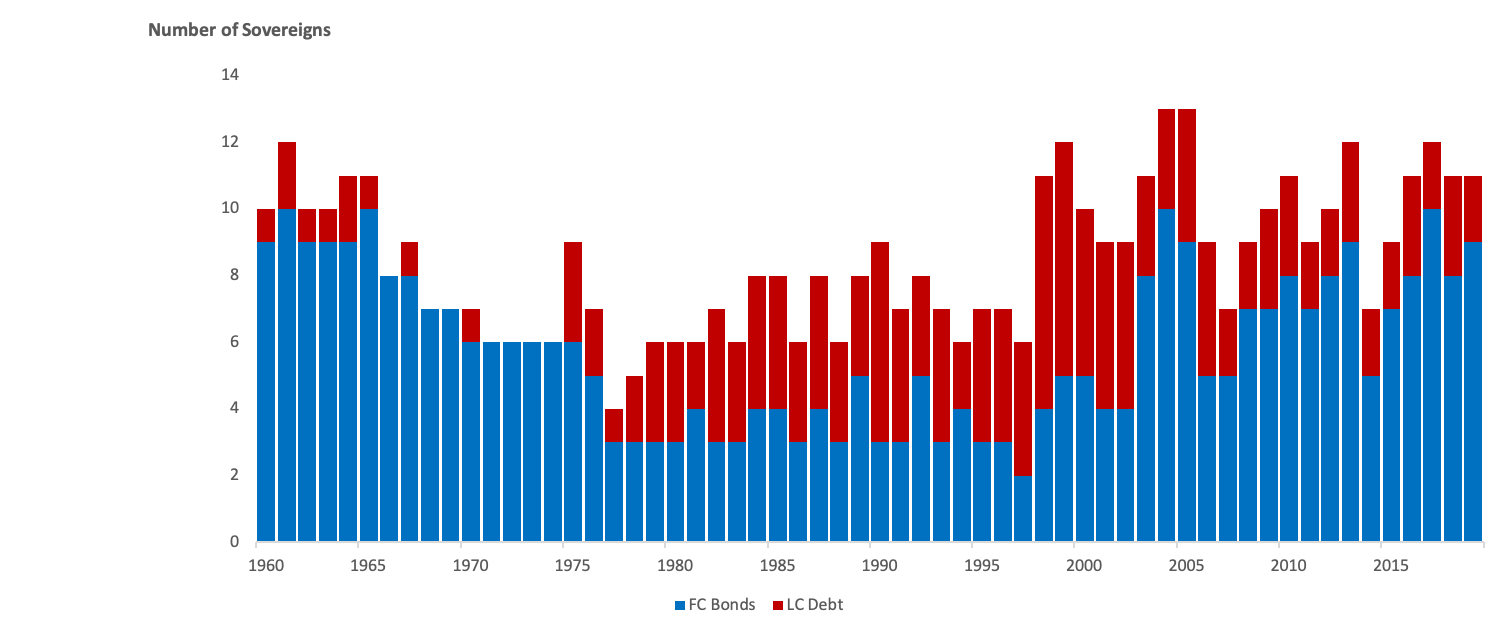
\includegraphics[width=0.85\textwidth,height=0.85\textheight]{../Figures/Slides/Defaults_FC_LC.png}
	\end{center}
	\begin{textblock*}{50mm}(23mm,83mm)
		\tiny Source: Beers, Jones and Walsh (2020).
	\end{textblock*}
\end{frame}
\note{A long-held view among some market participants is that governments rarely default on LC sovereign debt b/c they can print money}
\note{Figure: Defaults on LC debt do occur and are more common than is usually thought.
It is true that LC defaults are less frequent than FC defaults but the risk is there.
In fact, the number of domestic-law defaults has increased over time.
Since 1980 60+ default episodes under domestic law, bonds denominated in LC.
Examples of overt defaults in LC debt: Barbados (2018), Jamaica (2010, 2013), Nicaragua (2003, 2008), Argentina (2001), Turkey (1999) (earthquake, retroactively taxed LC debt), Russia (1998) after high inflation, Brazil 1990, Mexico 1982. El Salvador 2017, Cyprus 2013?

Important fact since debt denominated in LC has become an important source of funds for sovereigns and firms in EMs.

One of the points that I want to make is that this credit risk plays a risk in the bonds of EM.
}


\begin{frame}{.}
\begin{quote}
	``Overt \textit{de jure} defaults on domestic public debt \ldots are hardly rare.
\end{quote}
\begin{quote}
	The assumption embedded in many theoretical models that governments always honour the nominal face value of debt is a significant overstatement, particularly for emerging markets past and present."
\end{quote}
\begin{flushright}
	\textit{Reinhart and Rogoff (2011)}
\end{flushright}
\end{frame}
\note{Why LC defaults have limited visibility?
	- governments rarely acknowledge them. 
	- impacted investors are mostly domestic residents with limited avenues of redress. Since the pariticipation of foreign investment in sovereign LC debt instruments increased in the 90s increased awareness of more recent default cases.}
\note{Foreign investor participation has increased from 10\% in 2008 to 25\% in 2019.}
%\note{in 2011, G20 launched initiative to support LC bond markets in EM.}
%LC default unlikely for countries with debt mainly in LC at long maturity.


\begin{frame}
\frametitle{Credit Risk in Local Currency Yields}
\begin{center}
	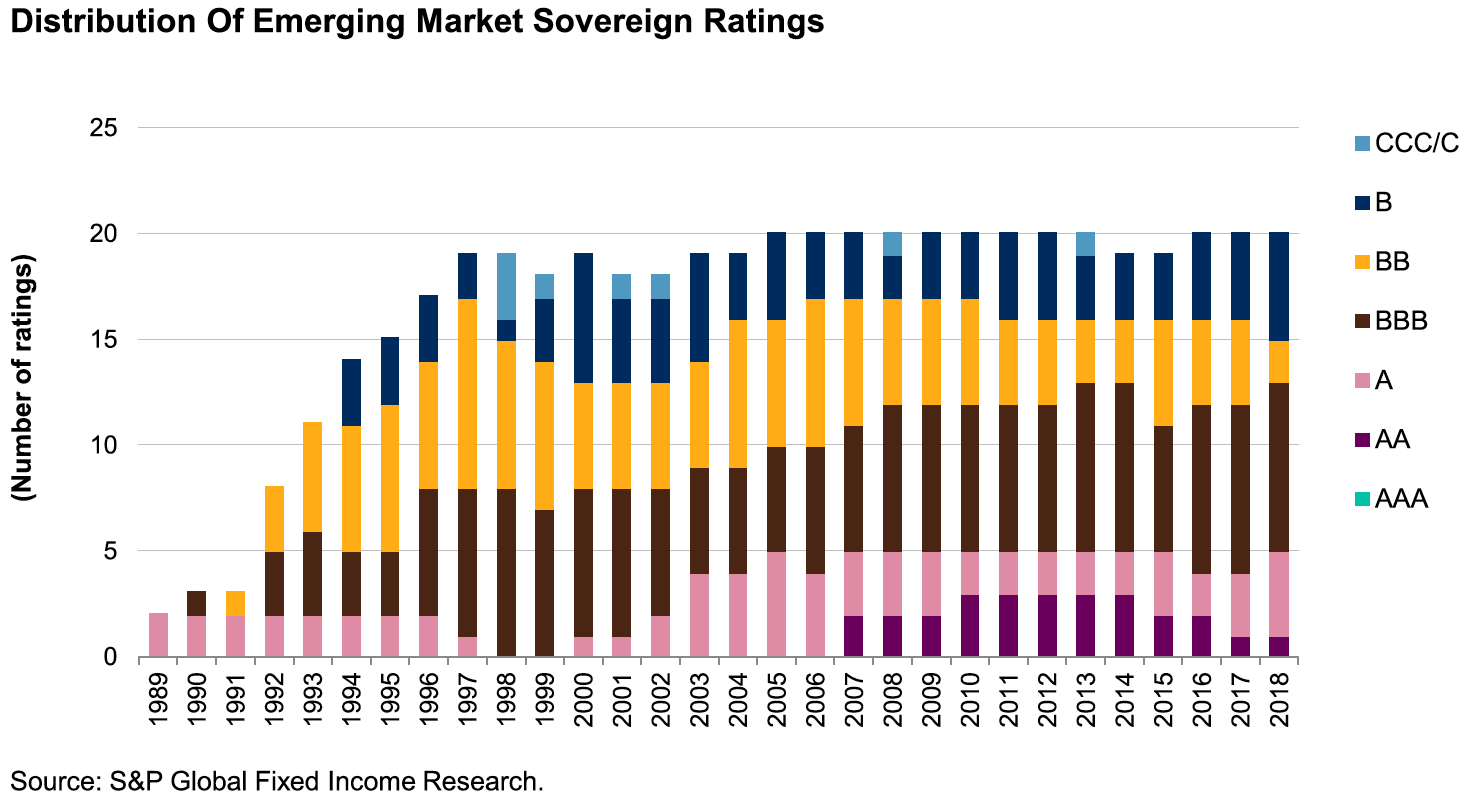
\includegraphics[width=0.8\textwidth,height=0.9\textheight]{../Figures/Slides/EM_LC_Ratings.png}
\end{center}
\end{frame}
%\note{Unlike AEs, credit risk in LC yields of EMs, even though they can print LC.}
\note{Reflected in the credit ratings of LC bonds.}
\note{Figure: EM sovereing ratings. They include Argentina, Brazil, China, Colombia, Egypt, Hungary, India, Indonesia, Lebanon, Malaysia, Mexico, Pakistan, Philippines, Poland, Qatar, Russia, Saudi Arabia, South Africa, Thailand, Turkey.}
\note{A bond is considered investment grade if its credit rating is BBB- or higher.}
\note{The are several countries with a rating below investment grade and none has a AAA rating.}
%\note{Credit risk broadly defined: (selective) default risk, currency convertibility risk, regulation risk, capital controls, jurisdiction risks, liquidity risk, sovereign restructurings.}


\begin{frame}
\frametitle{Stylized Yield Curve Decomposition}
\begin{center}
	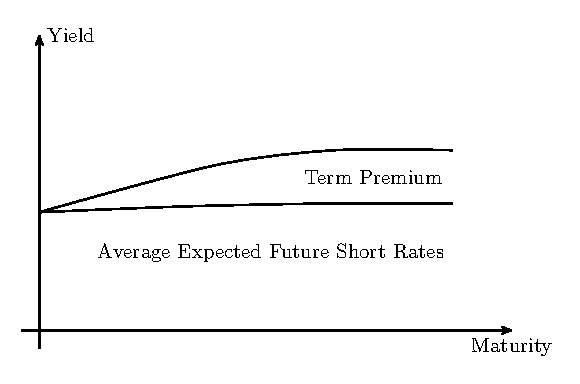
\includegraphics[trim={0cm 0cm 0cm 0cm},clip,width=0.85\textwidth,height=0.95\textheight]{../Figures/YC/ycdcmp_AE}
%	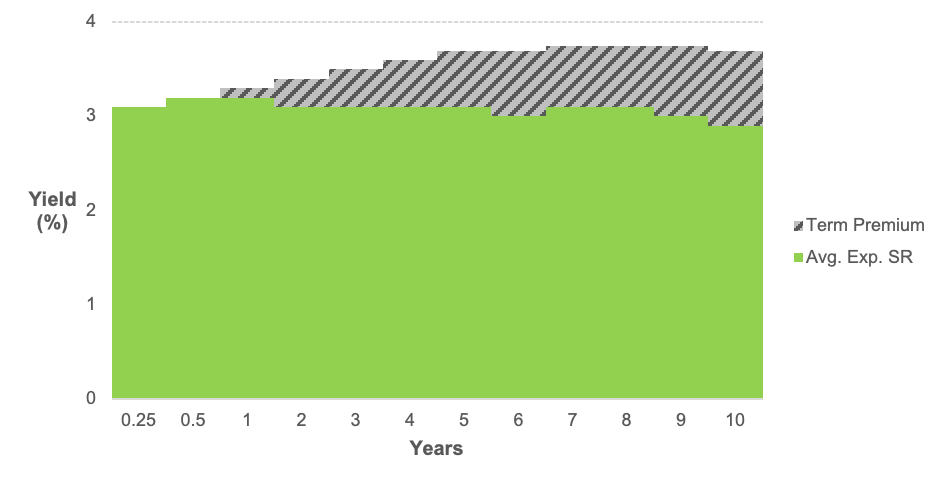
\includegraphics[trim={0cm 0cm 0.1cm 0cm},clip,width=0.85\textwidth,height=0.95\textheight]{../Figures/Slides/Yield_Dcmp_AE.png}
\end{center}
\end{frame}
\note{Figure: Stylized Yield Curve Decomposition. Two parts Avg Exp SR and TP.}
\note{Credit risk means that traditional decompositions of yield are not suitable for EM.}


\begin{frame}
	\frametitle{Research Questions}
	How to \alert{decompose} sovereign yields of emerging markets (EM)?
	\newline
	
	How does U.S. monetary policy \alert{transmit} to EM yields?
	\begin{itemize}
		\item Does it influence expectations of future policy rates? 
		\item Does it affect the term premium?
		\item Does it impact creditworthiness?
		\newline
	\end{itemize}
%	\begin{textblock*}{3cm}(.85\textwidth,0.85\textheight)
%		\hyperlink{LitReview}{\beamergotobutton{Related Literature}}
%	\end{textblock*}
	Understanding transmission channels \(\rightarrow\) \alert{Mitigate} undesired impacts
\end{frame}
\note{Quantify transmission channels of U.S. monetary policy to EM yields}
\note{Inform effective mitigation of undesired domestic impacts.}
%\note{Not only whether they comove but what drives the comovement.}
%\note{New perspective on the GFCy: financial conditions interrelated across countries.}
%\note{Better understanding of vulnerabilities in global financial system.}
%\note{These questions have barely received attention in the literature.}


\begin{frame}
\frametitle{Average EM Yield Curve Decomposition}
\begin{center}
	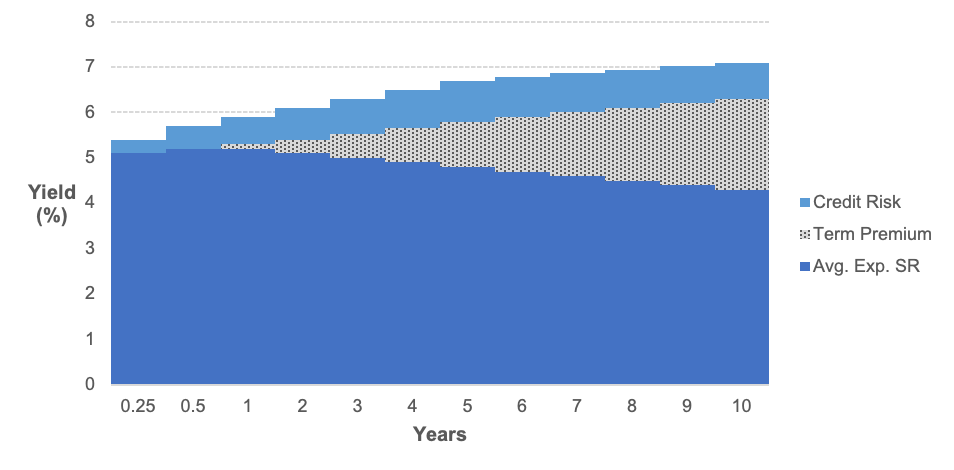
\includegraphics[trim={0cm 0cm 0.1cm 0cm},clip,width=0.85\textwidth,height=0.95\textheight]{../Figures/Slides/Yield_Dcmp_EM.png}
\end{center}
\end{frame}


\begin{frame}
	\frametitle{U.S. Monetary Policy Spillovers}
	\begin{enumerate}
		\item EM yields' response is economically significant, yet delayed over days
		\newline
		\item All three components react
		\begin{itemize}
			\item Reassessment of policy rate expectations
			\item Repricing of interest and credit risks
			\newline
		\end{itemize} 
		\item Unconventional measures limit EM monetary autonomy along the yield curve
	\end{enumerate}
\end{frame}

\begin{frame}[label=LitReview]
	\frametitle{Related Literature}
	
	\alert{Synthetic yields} and covered interest rate parity deviations
	\begin{itemize}
		\item {\footnotesize Du-Schreger (2016), Du-Im-Schreger (2018), Du-Tepper-Verdelhan (2018)}
	\end{itemize}

	\alert{Sovereign default} in EM local currency bonds
	\begin{itemize}
		\item {\footnotesize Reinhart-Rogoff (2011), Du-Schreger (2016), Erce-Mallucci (2018), \\ Otonello-Pérez (2019)}
	\end{itemize}
	
	\alert{Spillovers} of U.S. monetary policy to EM yields
	\begin{itemize}
		\item {\footnotesize Hausman-Wongswan (2011), Bowman-Londono-Sapriza (2015), Curcuru-Kamin-Li-Rodríguez (2018), Albagli-Ceballos-Claro-Romero (2019), Adrian-Crump-Durham-Moench (2019)}
	\end{itemize}
\end{frame}
\note{Point out three things.}
\note{International comparison of bond yields has focused on AEs.}
\note{LC debt overlooked by the (theoretical and empirical) literature until recently.}


\section{Yield Curves}


\begin{frame}
\frametitle{\alert{Nominal} Yield Curves}

	Local currency (LC) nominal yield curves (\(\yLCnom\)) from:
	\begin{itemize}
		\item Bloomberg Fair Value par yield curves \(\rightarrow\) Zero-coupon yield curves
	\end{itemize}
	
	But \alert{credit risk} embedded in LC nominal yields of \alert{EM} % ($\yLCnom$)
	
	\textbf{Approach}: Synthetic LC yields can be treated as \textit{free of credit risk}
	\begin{itemize}
		\item Swap U.S. Treasury yields into LC using currency derivatives
		\item Why not CDS (credit default swaps)?
	\end{itemize}
\end{frame}
\note{Sovereign debt of AEs is considered free of credit risk.}
%\note{Synthetic instead of nominal yields.}
\note{Under this approach, US YC used as a benchmark for all EMs.}
\note{CDS do not adequately characterize LC credit risk because defaults on LC bonds governed under domestic law are not triggers of CDS.}
%\note{Broad perspective on credit risk, i.e. not receiving promised payments: EMs can change the law + Suspension of currency convertibility + Capital controls + Actual default.}
%\note{BFV curves are par yield curves provided by Bloomberg on a daily basis for different maturities. To obtain the implied zero-coupon curves, the yields are converted into discount factors, which are then used to estimate the parameters of the Nelson-Siegel-Svensson model.}
%\note{CDS is a financial derivative that enable investors to swap credit risk.}


\begin{frame}[label=Synthetic]
\frametitle{\alert{Synthetic} Yield Curves}
%\vspace{-1cm}
\begin{equation*} \label{eq:uLCsynt}
	\eqyLCsynt
\end{equation*}
%\vspace{-0.5cm}

	\(\yLCsynt\): \(\tnr\)-period zero-coupon \textit{synthetic} yield of a country in LC at time $t$
	
	\(\yUS\): \(\tnr\)-period zero-coupon yield of the U.S. in USD at time \(\idxt\)
	
	\(\fwdprm\): \(\tnr\)-period \alert{forward premium} from USD to LC at time \(\idxt\)
%	\begin{itemize}
%		\item Currency forwards (\(< 1\) year) and cross-currency swaps (\(\geq 1\) year)
%	\end{itemize}
	
	\begin{itemize}
		\item \alert{\(< 1\) Year}: Currency forwards
		\[(forward_{t,\tnr} - spot_{t})/\tnr\]
		\item \alert{\(\geq 1\) Year}: Fixed-for-fixed cross-currency swaps
		%	\iftoggle{long}{\pause}{}
		\begin{itemize}
			\item Cross-currency basis swaps
			\item Interest rate swaps
		\end{itemize}
	\end{itemize}
%	\begin{textblock*}{3cm}(.92\textwidth,0.74\textheight)
%		\hyperlink{FwdPrm}{\beamergotobutton{FP}}
%	\end{textblock*}
\end{frame}
\note{FP compensates for the depreciation of the LC.}
\note{Notice that the nominal YC is not needed to get the synthetic YC.}
\note{Today I can lock in a risk-free investment in LC by 
exchanging LC for USD, investing those USD in Tresuaries and enter into a forward contract agreeing to sell USD for LC in the future. Once I receive the payment from Treasuries, I exchange it back into LC.
Don't need data on LC nominal yields to construct the synthetic yield.
Spread b/w LCNOM and LCSYNT is the CRC
}
\note{Currency forwards liquid up to 1Y.}
\note{Fixed-for-fixed XCS not directly traded in the market but they can be constructed.}
\note{CCS and IRS are liquid and collateralized. Bilateral counterparty risk is small.}


\begin{frame}
\frametitle{Cash Flow Diagram}
\begin{center}
	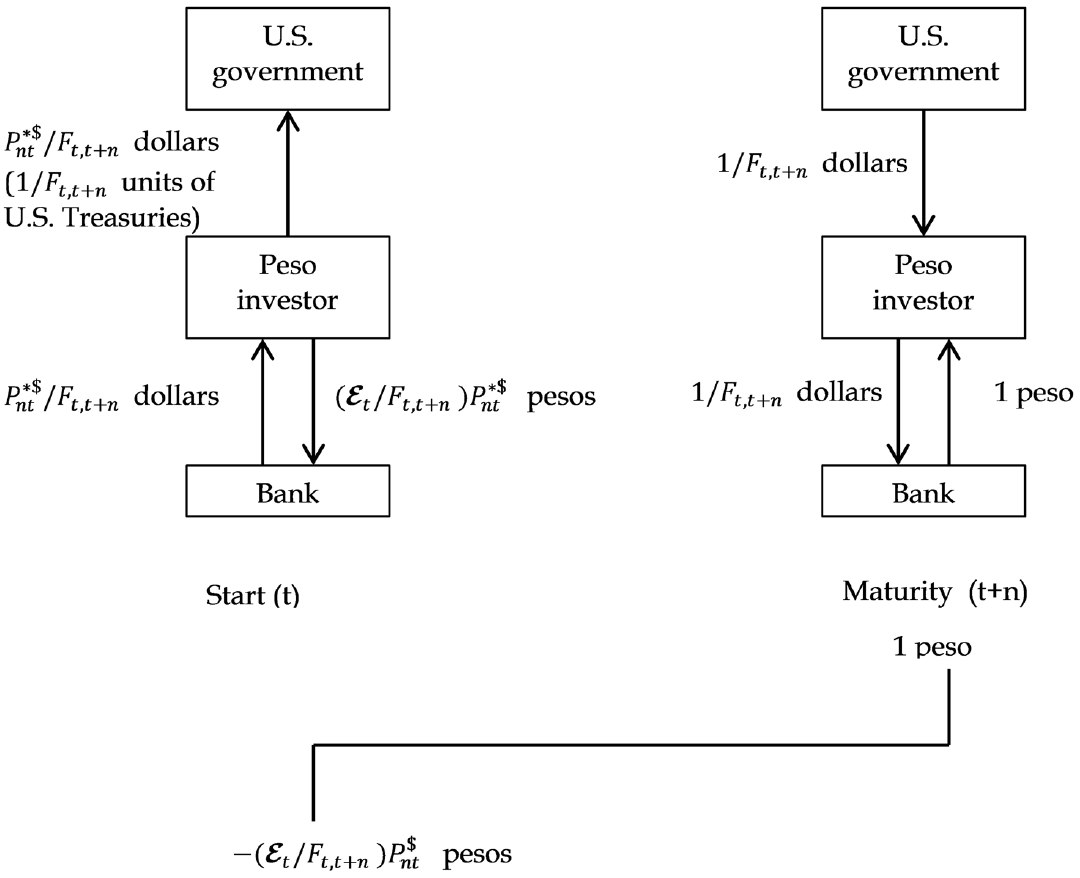
\includegraphics[width=0.85\textwidth,height=0.83\textheight]{../Figures/Slides/Cash_Flow_Diagram_Synthetic_LC.png}
\end{center}
\begin{textblock*}{50mm}(23mm,83mm)
	\tiny Source: \cite{DuSchreger:2016JoF}
\end{textblock*}
\end{frame}


\begin{frame}
\frametitle{Benchmark}

Assumptions:
\begin{enumerate}[(i)]
	\item Unconstrained arbitrageurs have access to U.S. and LC bonds
	\item Derivatives have no counterparty risk
	\item U.S. yields are free of default risk
\end{enumerate}

\cite{DuSchreger:2016JoF} show it is a \alert{useful benchmark}
\end{frame}


\begin{frame}[label=DevCIP]
\frametitle{Deviations from CIP (Covered Interest Parity)}
%\vspace{-1cm}
\[\eqCIPdevDS\]

	Measures:
	\begin{itemize}
		\item \alert{Sovereign credit risk} in EM
		\item[] \cite{DuSchreger:2016JoF} % (Du-Schreger '16)
		\item \alert{Convenience yield} for advanced countries (AE)
		\item[] \cite*{DuImSchreger:2018JIE} % (Du-Im-Schreger '18)
		\item Financial market \alert{frictions} for banks 
		\item[] \cite*{DuTepperVerdelhan:2018} % (Du-Tepper-Verdelhan '18)
	\end{itemize}
\end{frame}
\note{Diff b/w nominal and synthetic measures CIP deviations in government yields.}
\note{Correlation b/w CIP dev and CDS is high for EMs but not for AEs.}


\begin{frame}
\frametitle{Data}
	\alert{15 EM} countries:
	\begin{itemize}
%		\item[] {\scriptsize BRL, COP, HUF, IDR, ILS, KRW, MYR, MXN, PEN, PHP, PLN, RUB, THB, TRY, ZAR}
		\item Brazil, Colombia, Hungary, Indonesia, Israel, Korea, Malaysia, Mexico, Peru, Philippines, Poland, Russia, Thailand, Turkey, South Africa
	\end{itemize}
	%	\begin{itemize}
	%		\item \scriptsize \alert{10 AEs}: AUD, CAD, CHF, DKK, EUR, GBP, JPY, NOK, NZD, SEK
	%	\end{itemize}
%	\iftoggle{struct}{\item<2->}{\item} 
	
	Daily data starting in January 2000 to January 2019
%	\iftoggle{struct}{\item<3->}{\item}
	
	Maturities (in years): 0.25, 0.5, 1, 2, \ldots, 10
%	\iftoggle{struct}{\item<4->}{\item}
	
	Sources for \alert{synthetic} yields:
	\begin{itemize}
%		\iftoggle{struct}{\item<5->}{\item}
		\item $\yUS$: CRSP Risk-Free Rates \(+\) \citet*{GSW:2007}
%		\vspace{-0.1cm}
%		\iftoggle{struct}{\item<6->}{\item}
		\item $\fwdprm$: Bloomberg \(+\) Datastream
	\end{itemize}
\end{frame}
\note{Currency identifier for each country is shown.}
\note{Results are compared against those obtained for 10 AEs.}
\note{Starting dates vary by country.}
\note{At least 10 years of data}
\note{Longer series desirable to pin down TP since unobserved. But >10Y reasonable.}
\note{U.S. yield curve from GSW database.}
\note{Treasury securities with less than one year to maturity are less actively traded than longer-maturity ones. CRSP data is thought to be more robust at the short end.}
%\note{Reasons for use monthly: VAR is a good approximation for monthly, adequate frequency if want to use macro data.}
%\note{Consensus Economics provides long-horizon forecasts for consumer inflation and real GDP growth but not for policy rates.}


\section{Affine Term Structure Model}

\begin{frame}[label=ATSM]
\frametitle{Model Overview}
	
	Standard discrete-time nominal affine term structure model
	\begin{itemize}
		\item Assumption: Default-free bonds \(\rightarrow\) \alert{Synthetic} yields (\(\yLCsynt\)) for EM
		\item \alert{Augmented} with survey data
	\end{itemize}
	
	A set of pricing factors \(\Xvars\) drives the dynamics of the term structure
	
	No-arbitrage restrictions ensure consistency in cross section / time series %of yields
	
	Yields are affine functions of the pricing factors
	
%	\begin{textblock*}{3cm}(.89\textwidth,0.82\textheight)
%		\hyperlink{Qdynamics}{\beamergotobutton{Q Dynamics}}
%	\end{textblock*}
%	\begin{textblock*}{3cm}(.89\textwidth,0.88\textheight)
%		\hyperlink{Pdynamics}{\beamergotobutton{P Dynamics}}
%	\end{textblock*}
%	\begin{textblock*}{3cm}(.89\textwidth,0.94\textheight)
%		\hyperlink{Components}{\beamergotobutton{Decomposition}}
%	\end{textblock*}
\end{frame}
\note{ATSM standard tool to estimate dynamics of risk-free \alert{nominal} yield curves.}
\note{Coefficients: functions of the bond maturity and parameters of the model.}
\note{Once parameters estimated, decompose yields into expected short rate and TP.}
\note{Assumption yields are risk-free.}
\note{Decomposition into: YP and TP.}
%\note{The coefficients are functions of the maturity of the bond and the coefficients that determine the stochastic processes that drive the state variables.}


\begin{frame}
\frametitle{Bond Pricing}
Under no arbitrage, there exists a stochastic discount factor \(\SDF\) that prices all nominal bonds

Bond price today
	\begin{equation*} \label{eq:uPzeroP}
	\PzeroP 
\end{equation*}
	
There exists a theoretical risk-neutral pricing measure \(\Qmeasure\) defined as
	\begin{equation*} \label{eq:uPzeroQ}
	\PzeroQ 
\end{equation*}

\end{frame}


\begin{frame}[label=Qdynamics]
\frametitle{Dynamics Under \(\Qmeasure\) Measure}

Pricing factors under risk-neutral measure \(\Qmeasure\)
\begin{equation*} \label{eq:uXvarsQ}
	\eqXvarsFwdQ 
\end{equation*}

One-period interest rate
\begin{equation*} \label{eq:uShortRate}
	\eqshortrate 
\end{equation*}

Bond prices % is an exponentially affine function of the pricing factors
\begin{equation*}
	\Pzero = \exp\left( \affineA + \affineB \Xvars \right) ,
\end{equation*}

Fitted yields and loadings
\begin{equation*}
	\eqyZeroQ
\end{equation*}

%	\yZeroQ = \affineA^{\Qmeasure} + \affineB^{\Qmeasure} \Xvars

%\begin{textblock*}{3cm}(.92\textwidth,0.13\textheight)
%	\hyperlink{ATSM}{\beamergotobutton{Overview}}
%\end{textblock*}
\end{frame}

\begin{frame}[label=Pdynamics]
\frametitle{Dynamics Under \(\Pmeasure\) Measure}

Stochastic discount factor
\begin{equation*} \label{eq:uSDF}
	\eqSDF 
\end{equation*}

Market prices of risk
\begin{equation*} \label{eq:uRiskprice}
	\eqriskprice 
\end{equation*}

Pricing factors under physical measure \(\Pmeasure\)
\begin{equation*} \label{eq:uXvarsP}
	\eqXvarsFwdP
\end{equation*}

%\begin{textblock*}{3cm}(.92\textwidth,0.13\textheight)
%\hyperlink{ATSM}{\beamergotobutton{Overview}}
%\end{textblock*}
\end{frame}

\begin{frame}[label=Components]
\frametitle{EM Yield Decomposition}

Future expected short rate as if investors were risk-neutral (\(\lambdazero = \lambdaone = 0\))
\begin{equation*}
	\yZeroP = \affineAP + \affineBP \Xvars,
	%\yZeroP = - \frac{\affineA}{\tnr} - \frac{\affineB}{\tnr} \Xvars = \affineA^{\Pmeasure} + \affineB^{\Pmeasure} \Xvars,
\end{equation*}
\begin{center}
	\(\affineAP = - \frac{1}{\tnr} \affineA\), \(\affineBP = - \frac{1}{\tnr} \affineB\), \(\affineA = A(\deltazero, \deltaone, \XmuP, \XPhiP, \XSigma, \tnr)\) and \(\affineB = \mathcal{B}(\deltaone, \XPhiP, \tnr)\)
\end{center}


Term premium
\begin{equation*} \label{eq:uTPatsm}
	\termprm = \yZeroQ - \yZeroP.
\end{equation*}

Credit risk compensation
\[\CIPdev = \yLCnom - \yZeroQ\]

%\begin{textblock*}{3cm}(.92\textwidth,0.13\textheight)
%\hyperlink{ATSM}{\beamergotobutton{Overview}}
%\end{textblock*}
\end{frame}
\note{Synthetic curve better aligns with the risk-free assumption.}
\note{ATSM for synthetic allows to decompose nominal into 3 parts.}


\begin{frame}
\frametitle{Weak Identification}

Yield data accurately identifies \{\(\XmuQ, \XPhiQ\)\}, yet \{\(\XmuP, \XPhiP\)\} \alert{poorly} identified
\begin{itemize}
	\item Bond yields are persistent
	\item Unstable yield decompositions
\end{itemize}

\textbf{\alert{Solutions}}: Survey data, parameter restrictions, bias-corrected estimators

\cite{Guimaraes:2014}: Surveys provide \alert{robust} decompositions of yields
\begin{itemize}
	\item Surveys anchor the long run mean of interest rates
	\item Important for EM due to small sample sizes
\end{itemize}
%Most variability attributed to fluctuations in term premium
% Overestimates stability of expected path of short rate

\end{frame}
\note{Poorly identified parameters under the \(\Pmeasure\) measure result in unstable yield decompositions.}
\note{Overestimates stability of expected path of short rate}
\note{Estimation requires long time series}
\note{Only ZC bond yields are needed to estimate ATSM parameters.}
\note{However, TP is an unobserved variable.}
\note{Uses of surveys: (1) model-free TP estimate. (2) supplement in ATSMestimation.}
%\note{Surveys are an effective solution to obtain robust decompositions of the yield curve \citep{Guimaraes:2014} 

\begin{frame}[label=SCBP]
\frametitle{Survey Data}

No data on long-term forecasts for the short rate in EM

Implied forecast for the short rate in EM from existing data %on long-term forecasts
\begin{itemize}
\item \alert{EM inflation expectations} from Consensus Economics (CE)
\begin{itemize}
	\item Twice a year
\end{itemize}

\item Implied \alert{U.S real rate} from Survey of Professional Forecasters (SPF)
\begin{itemize}
\item T-bill rate, CPI inflation
%\item Compared against TIPS yields
\end{itemize}
\end{itemize}

\begin{equation*} \label{eq:uRrt}
	\eqrrt
\end{equation*}

%\begin{textblock*}{3cm}(.87\textwidth,0.47\textheight)
%	\hyperlink{SvyAugModel}{\beamergotobutton{Implied Forecast}}
%\end{textblock*}
\end{frame}
\note{Rely on the SEO assumption -> Fisher equation.}
\note{Use them in survey augmented model.}
\note{Data available twice a year.}


\begin{frame}[label=yldcbp]
%	\frametitle{Components: Expected Future Short Rate}
\begin{center}							% center the figure inside the minipage
	\includegraphics[trim={0cm 0cm 0cm 0cm},clip,height=0.95\textheight,width=\linewidth]{../Figures/Data/YLD10Y_CBP.eps} \\
\end{center}
%\begin{textblock*}{5cm}(0.97\textwidth,1.05\textheight)
%	\hyperlink{YldDcmp}{\beamerreturnbutton{Decomposition}}
%\end{textblock*}
\end{frame}


\begin{frame}[label=SvyAugModel]
\frametitle{Survey-Augmented Model}

Expected average short rate under \(\Pmeasure\)
\begin{equation*}
	\yZeroE = \frac{1}{\tnr} \ExpP \left[ \sum_{j=0} ^{\tnr-1} \srate_{\idxt+j} \right] = \affineAe + \affineBe \Xvars,
\end{equation*}

Forward rate from \(\tnr\) to \(\tnrfwd\) periods hence
\begin{equation*}
	\yZeroEfwd = \affineAeFwd + \affineBeFwd \Xvars.
\end{equation*}

%\begin{textblock*}{3cm}(.9\textwidth,0.14\textheight)
%	\hyperlink{SCBP}{\beamergotobutton{Survey Data}}
%\end{textblock*}
\end{frame}

\begin{frame}
\frametitle{Model Estimation}

%	\item Use \cite*{JSZ:2011} normalization of the model %: \(\Pmeasure \perp \Qmeasure\) % likelihood functions
Estimate parameters by MLE with monthly data
\begin{itemize}
\item \cite*{JSZ:2011} normalization of the model
\end{itemize}
%	\item Estimate \(\Pmeasure\) parameters by OLS
%	\item Estimate \(\Qmeasure\) parameters by MLE

Estimate survey-augmented model by Kalman filter (missing data)
\begin{itemize}
\item Surveys as \alert{`noisy'} expectations measures \citep{KimOrphanides:2012}
\end{itemize}

Standard errors by delta method

Estimate daily pricing factors

\end{frame}
\note{End-of-month data}


\section{EM Yield Decomposition}


\begin{frame}[label=ModelFit]
%	\frametitle{Model Fit}
\begin{center}							% center the figure inside the minipage
\includegraphics[trim={0cm 0cm 0cm 0cm},clip,height=0.95\textheight,width=\linewidth]{../Figures/Estimation/s_ylds_bsl_yQ.eps} \\
\end{center}
\end{frame}

\begin{frame}[label=YldDcmp]
%	\frametitle{Decomposition of EM Nominal Yields}
\begin{center}							% center the figure inside the minipage
\includegraphics[trim={0cm 0cm 0cm 0cm},clip,height=0.95\textheight,width=\linewidth]{../Figures/Estimation/ny_dcmp.eps} \\
\end{center}
%\begin{textblock*}{5cm}(.2\textwidth,1.08\textheight)
%\hyperlink{yPscbp}{\beamergotobutton{Average Expected Short Rates}}
%\end{textblock*}
\begin{textblock*}{3cm}(.51\textwidth,1.08\textheight)
\hyperlink{tpCI}{\beamergotobutton{Term Premia}}
\end{textblock*}
\begin{textblock*}{5cm}(.725\textwidth,1.08\textheight)
\hyperlink{crcCI}{\beamergotobutton{Credit Risk Compensation}}
\end{textblock*}
\end{frame}
\note{Dynamics of TP and LCCS important in EM bond yields.}
\note{EM TP estimates assessed against stylized facts for USTP.}
\note{Events: GR, TT, US election, 2009 QE1.}
\note{TP decline due to: international investors, US UMP.}
%\note{USTP increased around the onset of the Great Recession (September 2008), the taper tantrum (June 2013), and the 2016 U.S. presidential election (November 2016), while it declined after the first unexpected announcement of the QE program by the Fed (March 2009).}
%\note{Common explanations for the decline in the USTP include an increased demand of U.S. assets by global investors and the effects of the UMP of the Fed.}
%\note{Explanation for change in sign (Campbell, Sunderam \& Viceira (2016)): TP < 0 is explained by the flip in the sign of the correlation between stocks and bonds -bonds hedge stocks-.}

\begin{frame}[label=yPscbp]
%	\frametitle{Components: Expected Future Short Rate}
\begin{center}							% center the figure inside the minipage
	\includegraphics[trim={0cm 0cm 0cm 0cm},clip,height=0.95\textheight,width=\linewidth]{../Figures/Estimation/bsl_yP_scbp.eps} \\
\end{center}
%\begin{textblock*}{5cm}(0.97\textwidth,1.05\textheight)
%	\hyperlink{YldDcmp}{\beamerreturnbutton{Decomposition}}
%\end{textblock*}
\end{frame}

\begin{frame}[label=rrtLT]
%	\frametitle{Components: Expected Future Short Rate}
\begin{center}							% center the figure inside the minipage
	\includegraphics[trim={0cm 0cm 0cm 0cm},clip,height=1.05\textheight,width=\linewidth]{../Figures/Estimation/rrt_LTvsUSrrt.eps} \\
\end{center}
%\begin{textblock*}{5cm}(0.97\textwidth,1.05\textheight)
%	\hyperlink{YldDcmp}{\beamerreturnbutton{Decomposition}}
%\end{textblock*}
\end{frame}

\begin{frame}[label=tpUCSV]
\frametitle{Term Premium and Inflation Uncertainty}

Term premium compensates for \alert{inflation uncertainty} \citep{Wright:2011}
%In advanced countries related to inflation uncertainty \citep{Wright:2011} % in advanced countries

Inflation higher and more volatile in EM than AE \citep{HaKoseOhnsorge:2019}

Is inflation uncertainty more relevant to term premia in EM?

\begin{equation*} \label{eq:uPanelUCSV}
	\eqpanelUCSV ,
\end{equation*}

\begin{itemize}
	\item \(\sigma^{\pi}_{\idxspnl}\): standard deviation of permanent component of inflation in UCSV model \citep{StockWatson:2007}
\end{itemize}

\end{frame}

\begin{frame}
\frametitle{EM Term Premium and Inflation Uncertainty}
%	\setbeamercolor{background canvas}{bg=}
%	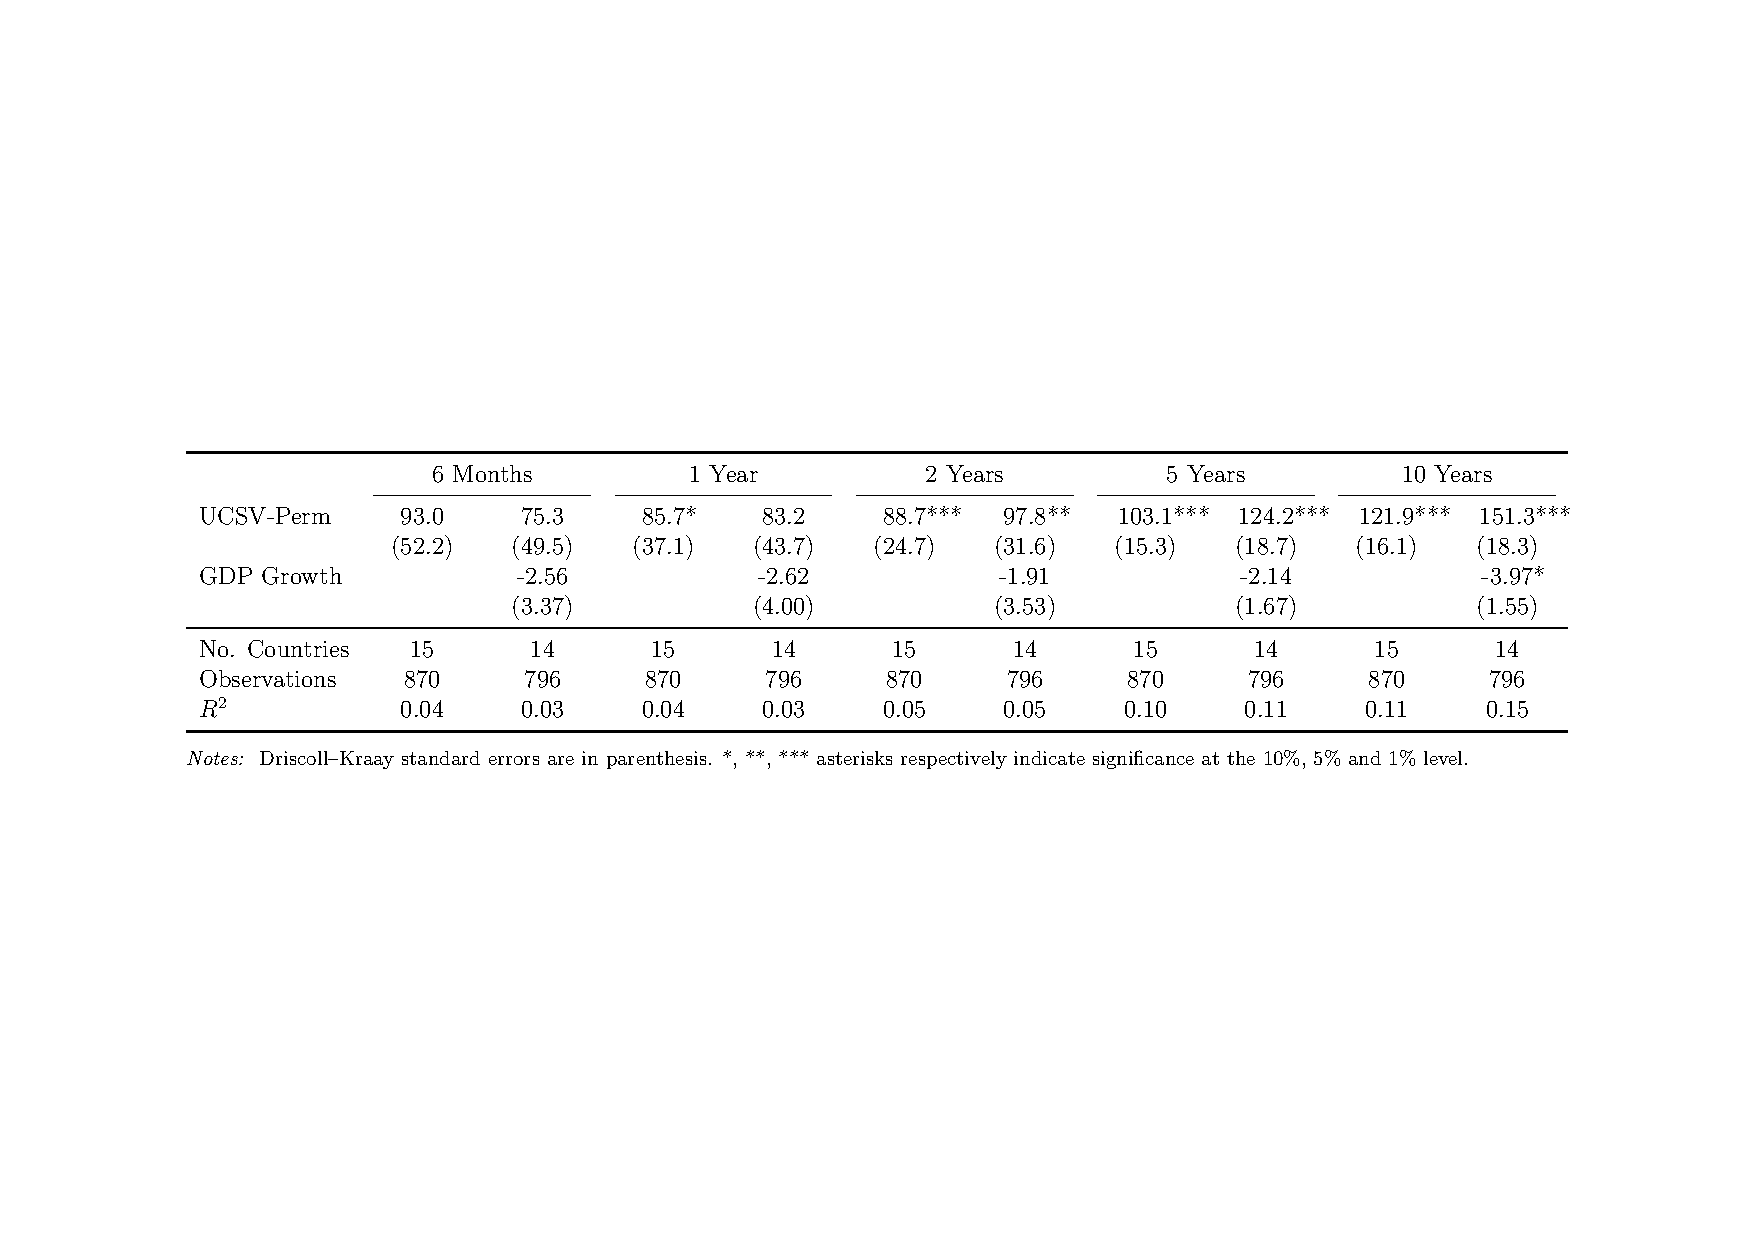
\includepdf[pages={1}]{../Tables/tpucsv.pdf}
\vspace{-0.8cm}
\begin{figure}[!htbp]
\begin{center} % trim removes: left, down, right, top
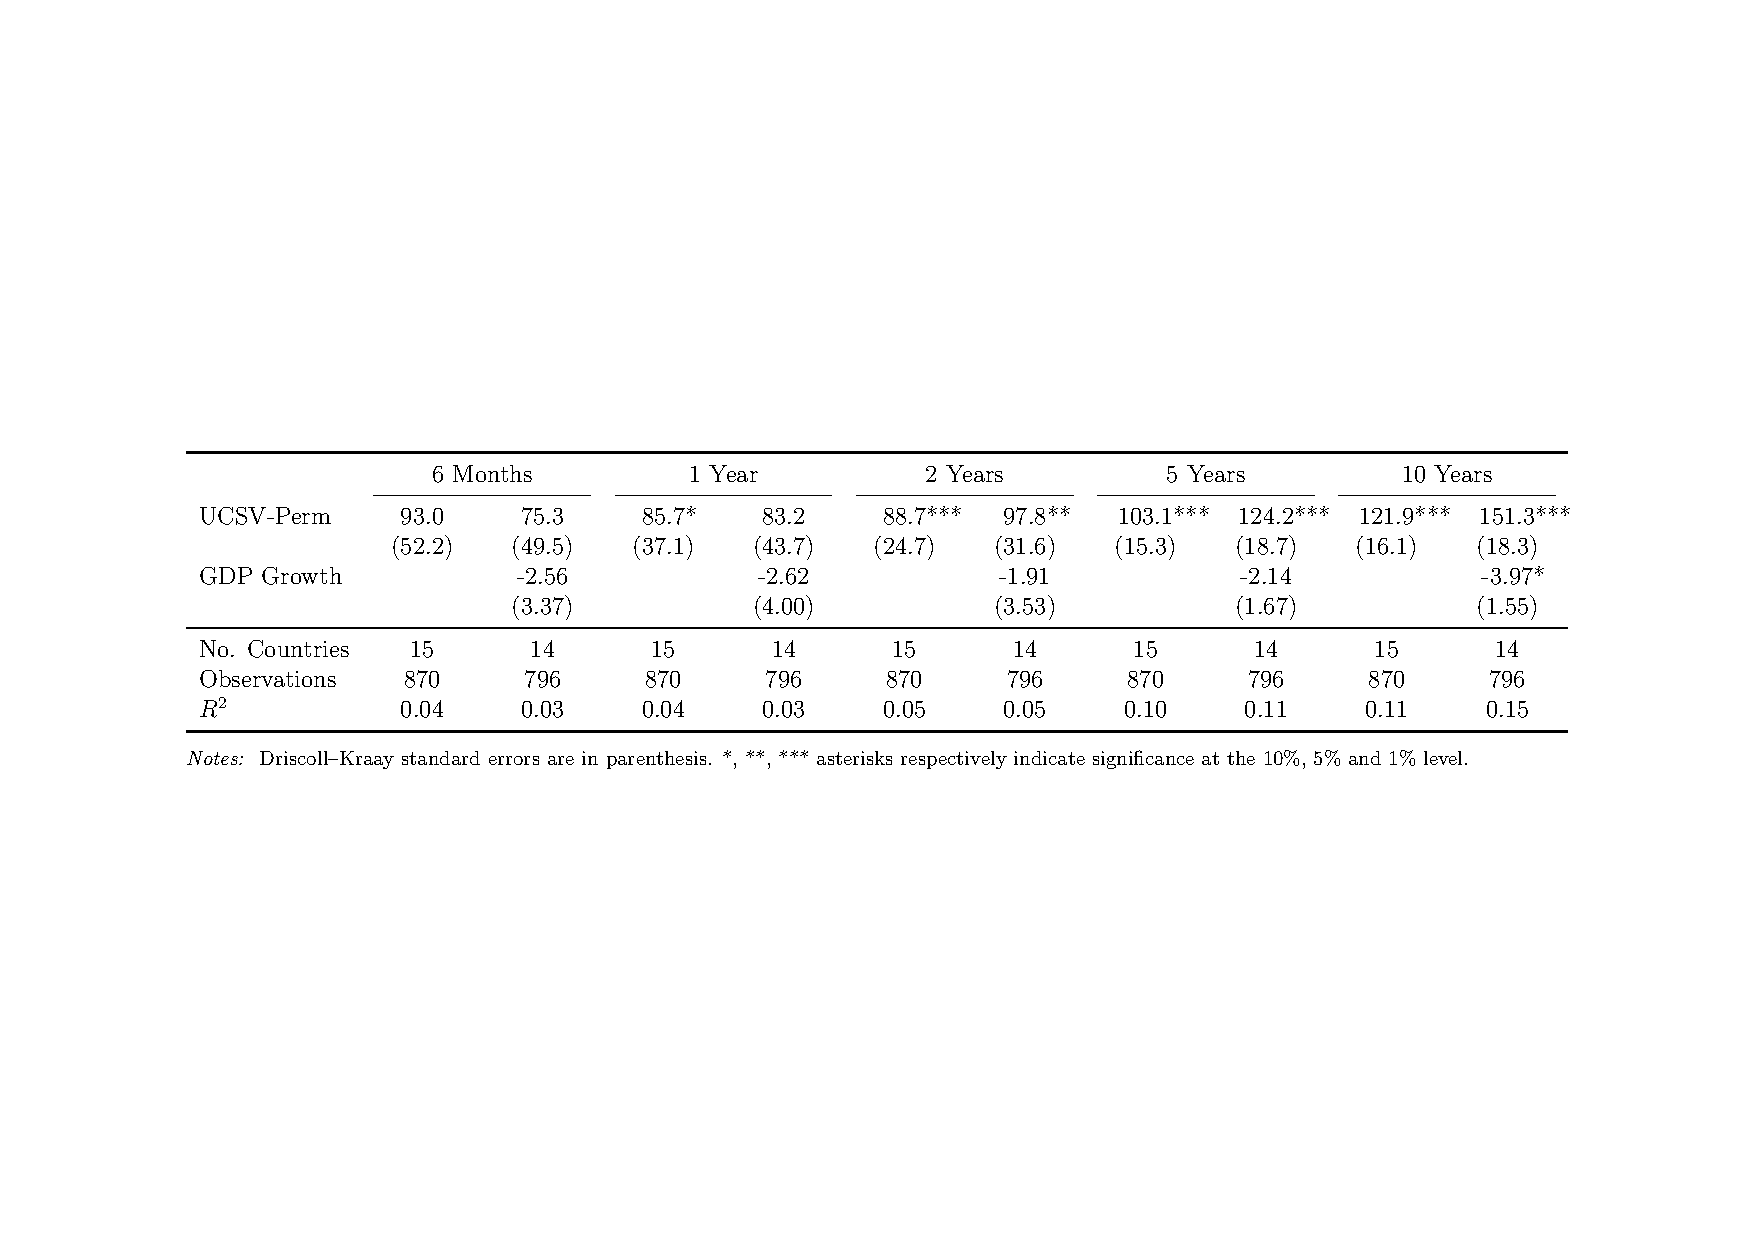
\includegraphics[trim={4cm 6cm 3cm 6.5cm},clip, width=1.05\textwidth,height=0.95\textheight]{../Tables/tpucsv.pdf}
\par\end{center}
\end{figure}
\end{frame}


\section{Spillovers}

\begin{frame}
\frametitle{The Yield Curve Channel}
Long-term yields highly correlated, influenced by global forces

Unconventional monetary policies abroad affect EM long-term yields
\begin{itemize}
	\item Via the term premium \citep{Turner:2014}
\end{itemize}

\alert{EM monetary autonomy}:
\begin{itemize}
	\item Declines along the yield curve \citep{Obstfeld:2015}
	\item Limited also at the short end \citep{Kalemli-Ozcan:2019}
\end{itemize}
\end{frame}

\begin{frame}
\frametitle{Yield Curve Channel Implications}

Do long-term EM yields \alert{comove} more than short-term ones?
\begin{itemize}
\item Rolling correlations % Connectedness index \citep{DieboldYilmaz:2014}
\end{itemize}

\alert{Direct} relationships at different maturities
\begin{itemize}
\item U.S. term premium \(\rightarrow\) EM term premium
\item U.S. expected future short rates \(\rightarrow\) EM expected future short rates
\end{itemize}

\alert{Cross} relationships at the short end
\begin{itemize}
\item U.S. term premium \(\rightarrow\) EM expected future short rates
\end{itemize}

\end{frame}
\note{Cross effect at 2Y maturity.}

%\begin{frame}[label=DYindex]
%\frametitle{EM Yields Comovement}
%\begin{figure}[!htbp]
%\begin{center} % trim removes: left, down, right, top
%\includegraphics[trim={0cm 0cm 0cm 0cm},clip,height=0.8\textheight,width=0.85\linewidth]{../Figures/Estimation/dy_index_dn_data.eps}
%\par\end{center}
%\end{figure}
%\begin{textblock*}{10cm}(45mm,83mm)
%\footnotesize Connectedness Index \citep{DieboldYilmaz:2014}
%\end{textblock*}
%\begin{textblock*}{5cm}(1.02\textwidth,0.55\textheight)
%	\hyperlink{RollingCorr}{\beamergotobutton{Rolling Corr.}}
%\end{textblock*}
%\end{frame}

\begin{frame}[label=RollingCorr]
\frametitle{EM Yields Comovement}
\begin{figure}[!htbp]
	\begin{center} % trim removes: left, down, right, top
		\includegraphics[trim={0cm 0cm 0cm 0cm},clip,height=0.8\textheight,width=0.85\linewidth]{../Figures/Estimation/rolling_dn_data.eps}
		\par\end{center}
\end{figure}
\begin{textblock*}{10cm}(67.5mm,83mm)
	\footnotesize Rolling Correlations
\end{textblock*}
\begin{textblock*}{5cm}(1.02\textwidth,0.55\textheight)
	\hyperlink{DYindex}{\beamergotobutton{D-Y Index}}
\end{textblock*}
\end{frame}

\begin{frame}
\frametitle{Is There A Yield Curve Channel?}
%\begin{itemize}
%	\item Panel regression:
%\vspace{-1cm}
\begin{equation*} \label{eq:uPanelDCMP}
	\eqpanelTPreg
\end{equation*}
%\vspace{-1cm}

\(\yld_{\idxspnl}\): nominal EM yields and their three components

\(\alpha_{i}\): country fixed effects

\(z^{1}_{\idxspnl}\): U.S. yield curve decomposition \citep{KimWright:2005}

\(z^{2}_{\idxspnl}\): Global and domestic drivers
\begin{itemize}
	\item Vix, EPU \citep{BakerBloomDavis:2016} \& global activity  \citep{Hamilton:2019} indexes
	\item Policy rate, inflation, unemployment, exchange rate (standardized) %(LC per USD)
\end{itemize}

%\end{itemize}
\end{frame}
\note{Country FE allow for the possibility that country-specific factors that may affect TP are also correlated with the controls.}

\begin{frame}
%	\frametitle{EM Term Premium and Inflation Uncertainty}
\vspace{-0.8cm}
\begin{figure}[!htbp]
\begin{center} % trim removes: left, down, right, top
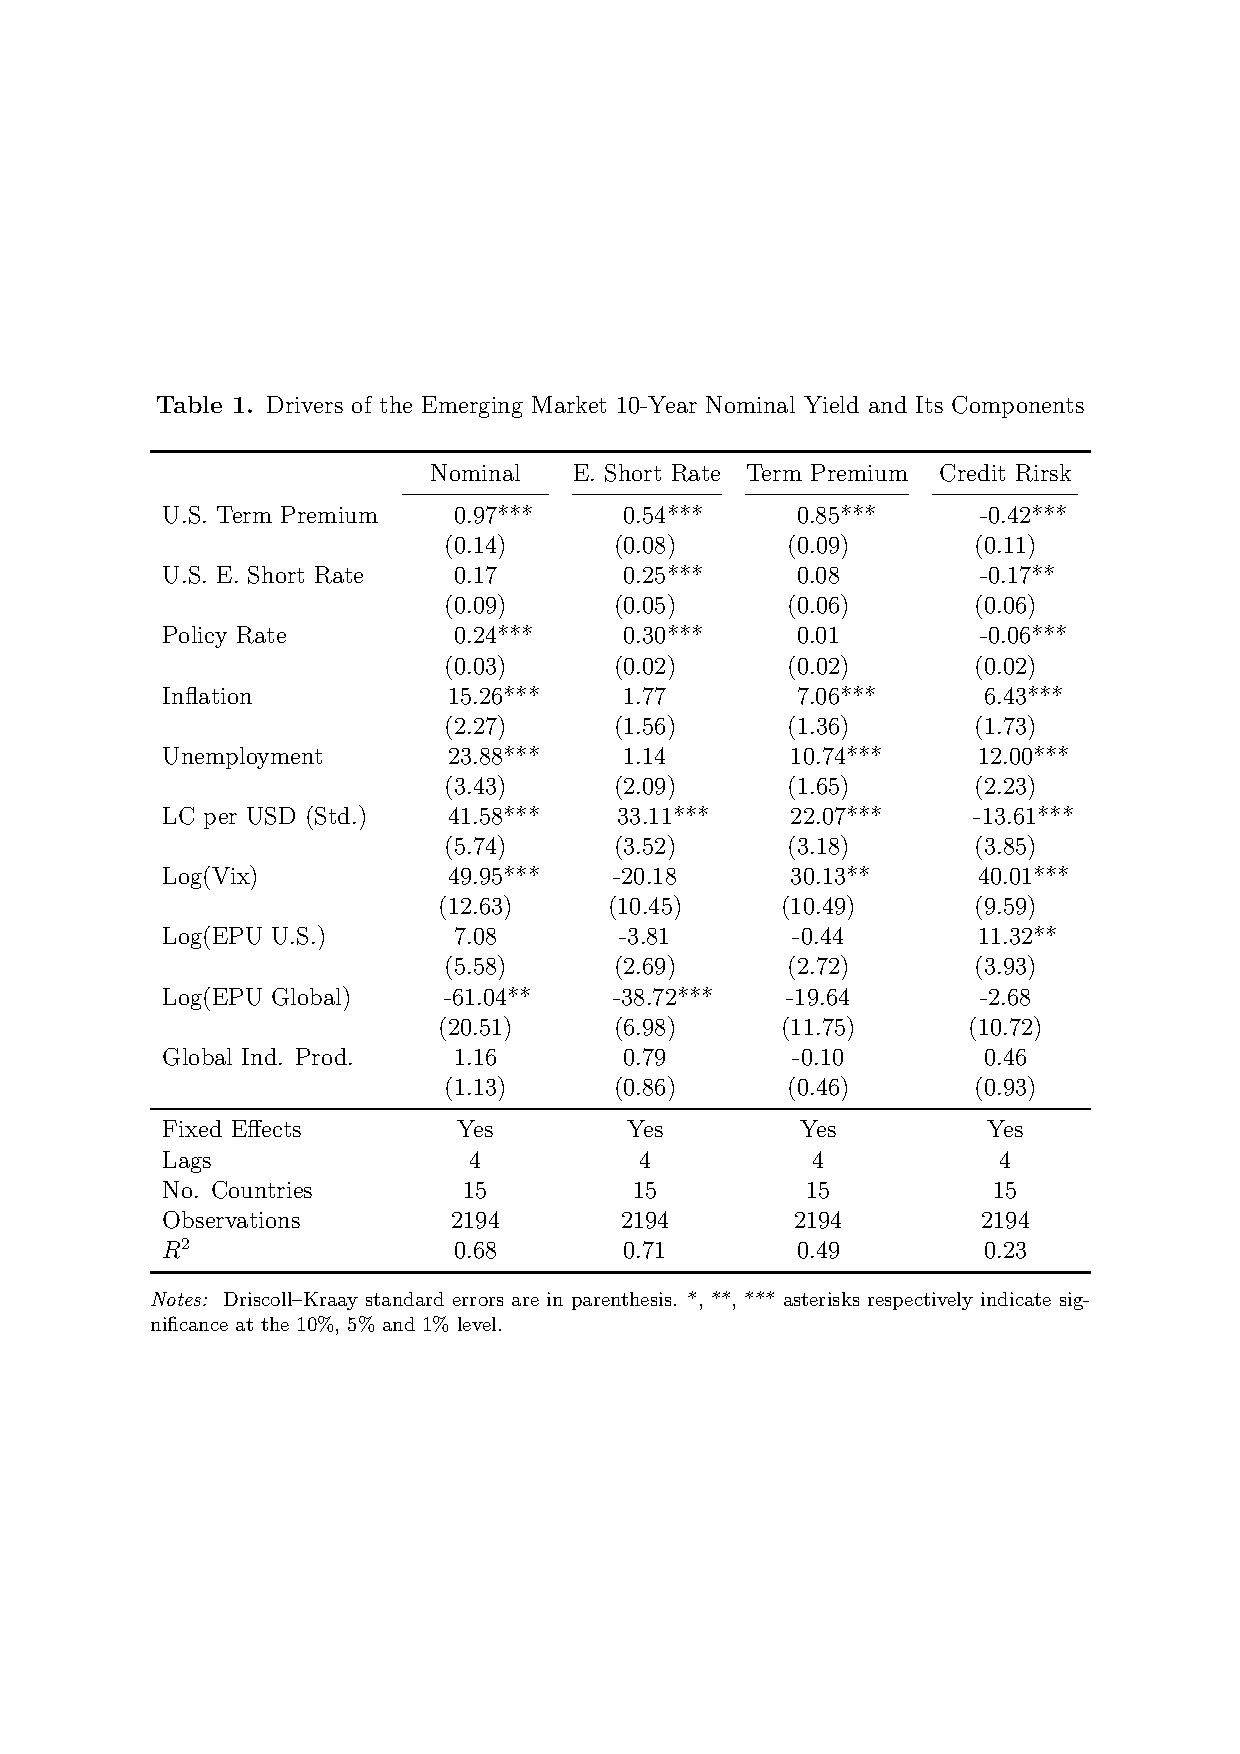
\includegraphics[trim={2cm 7.2cm 2cm 4cm},clip, width=0.95\textwidth,height=1.15\textheight]{../Tables/ycdcmp10y.pdf}
\par\end{center}
\end{figure}
\end{frame}

%\note{Confirms that external conditions impact domestic bond markets.}
%\note{US MP has effect not through FFR directly but via USTP.}
%\note{Effect of the domestic variables in line with findings for AEs.}
%\note{Higher TP during recessions: high UNE, low IP. Evidence of EM TP countercyclical.}
%\note{INF erodes value of nominal bonds: in periods of rising INF demand a higher TP.}
%\note{Higher TP due to FX depreciation in line with risk-taking channel of FX.
%	Currency depreciation tightens financial conditions, higher sovereign bond spreads.}
%\note{Main broad message at 10 years. Big difference: FFR more negative when there is no USTP and disappears when USTP.}
%\note{Effect of the domestic variables in line with findings for AEs. 
%	Investors demand a higher term premium during recessions, when the unemployment rate increases. This shows evidence of a countercyclical behavior of the TP in EMs.
%	The positive effect of inflation on the TP conforms with the idea that inflation erodes the value of nominal bonds and so in periods of rising inflation investors demand a higher TP.}
%\note{A depreciation of the LC is associated with an increase in the TP. This seems counterintuitive since EMs are usually commodity exporters so it appears to contradict the standard trade-channel effect. 
%	However, it is in line with the risk-taking channel of exchange rates found by \cite{HofmannShimShin:2017}, according to which currency depreciation is associated with tighter financial conditions and increased sovereign bond spreads.}


\begin{frame}
%	\frametitle{EM Term Premium and Inflation Uncertainty}
\vspace{-0.8cm}
\begin{figure}[!htbp]
\begin{center} % trim removes: left, down, right, top
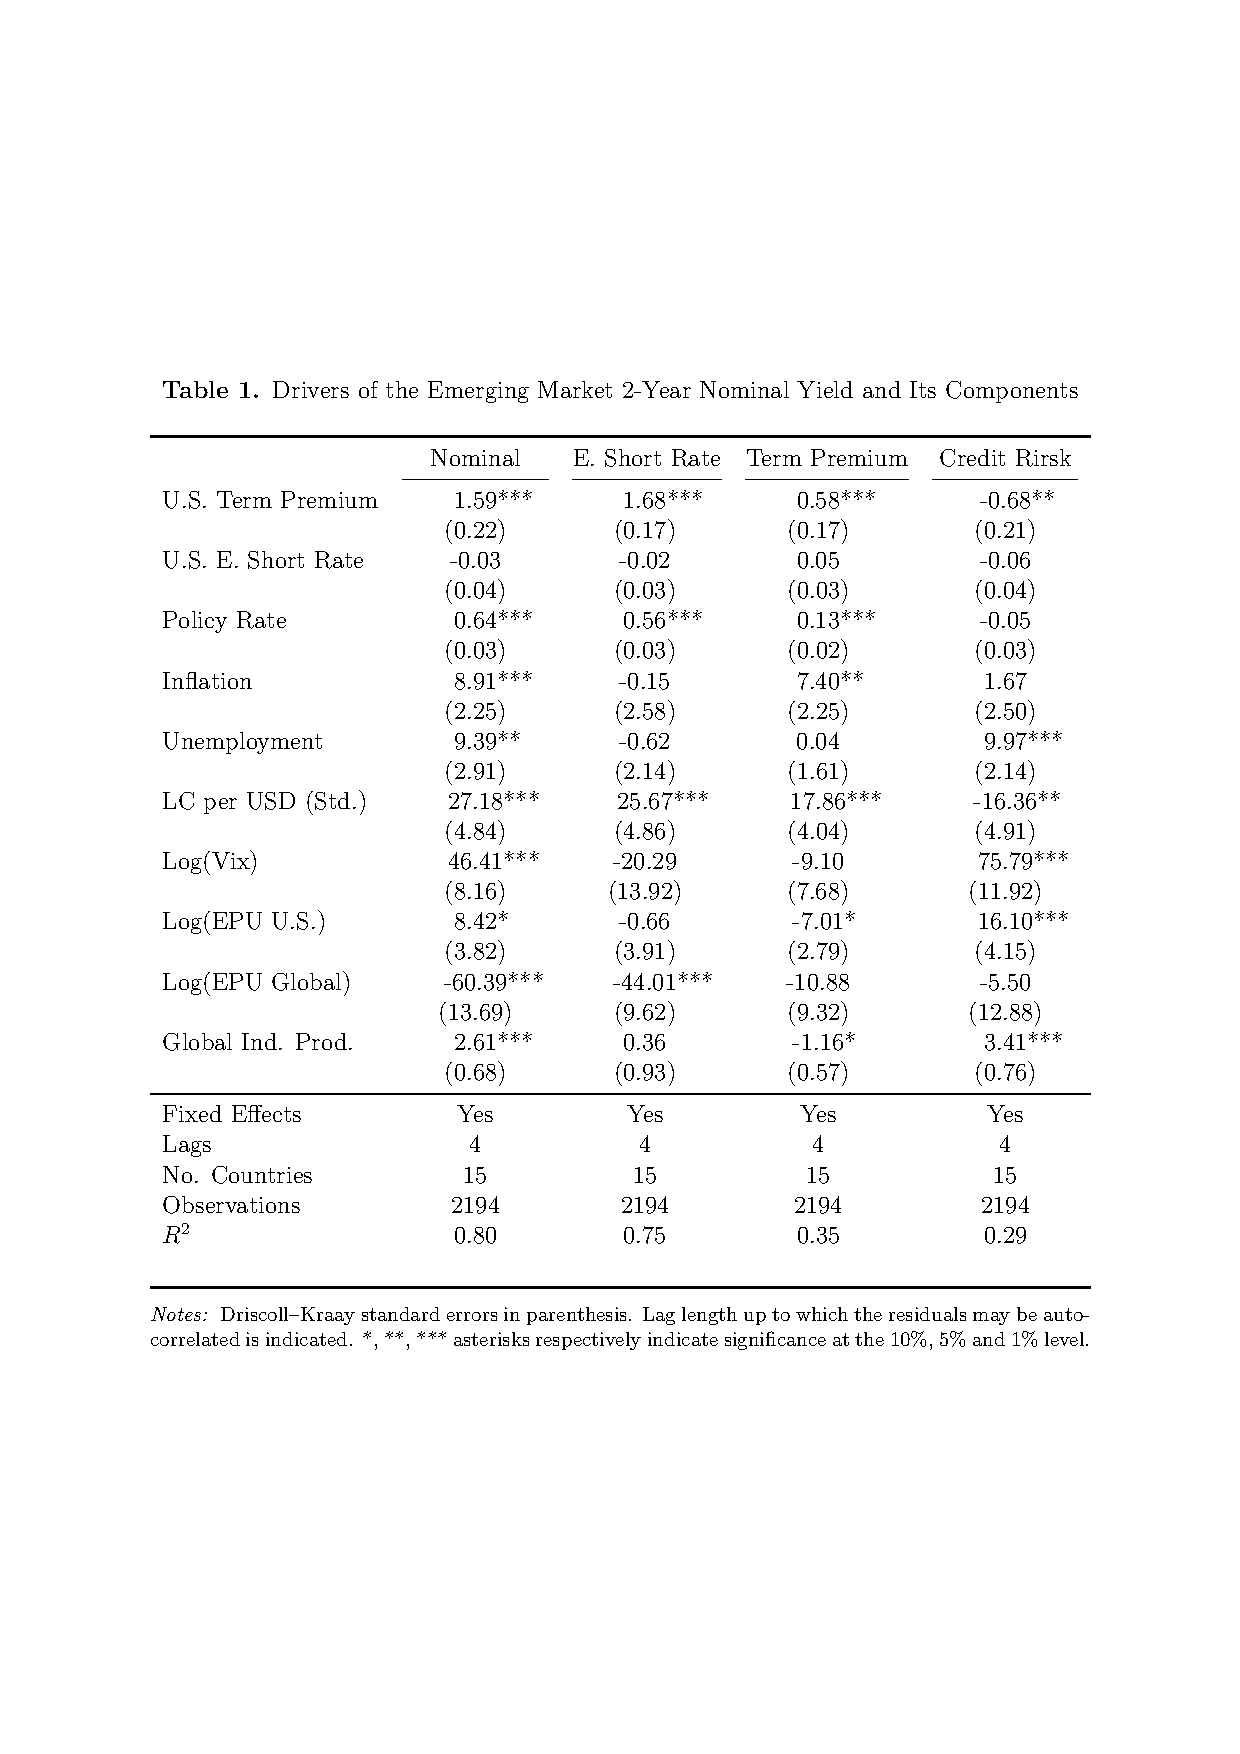
\includegraphics[trim={2cm 7.2cm 2cm 4cm},clip, width=0.95\textwidth,height=1.15\textheight]{../Tables/ycdcmp2y.pdf}
\par\end{center}
\end{figure}
\end{frame}

%\begin{frame}
%%	\frametitle{EM Term Premium and Inflation Uncertainty}
%\vspace{-0.8cm}
%\begin{center}
%	\begin{tikzpicture}
%	\node (table) at (0,0)
%	{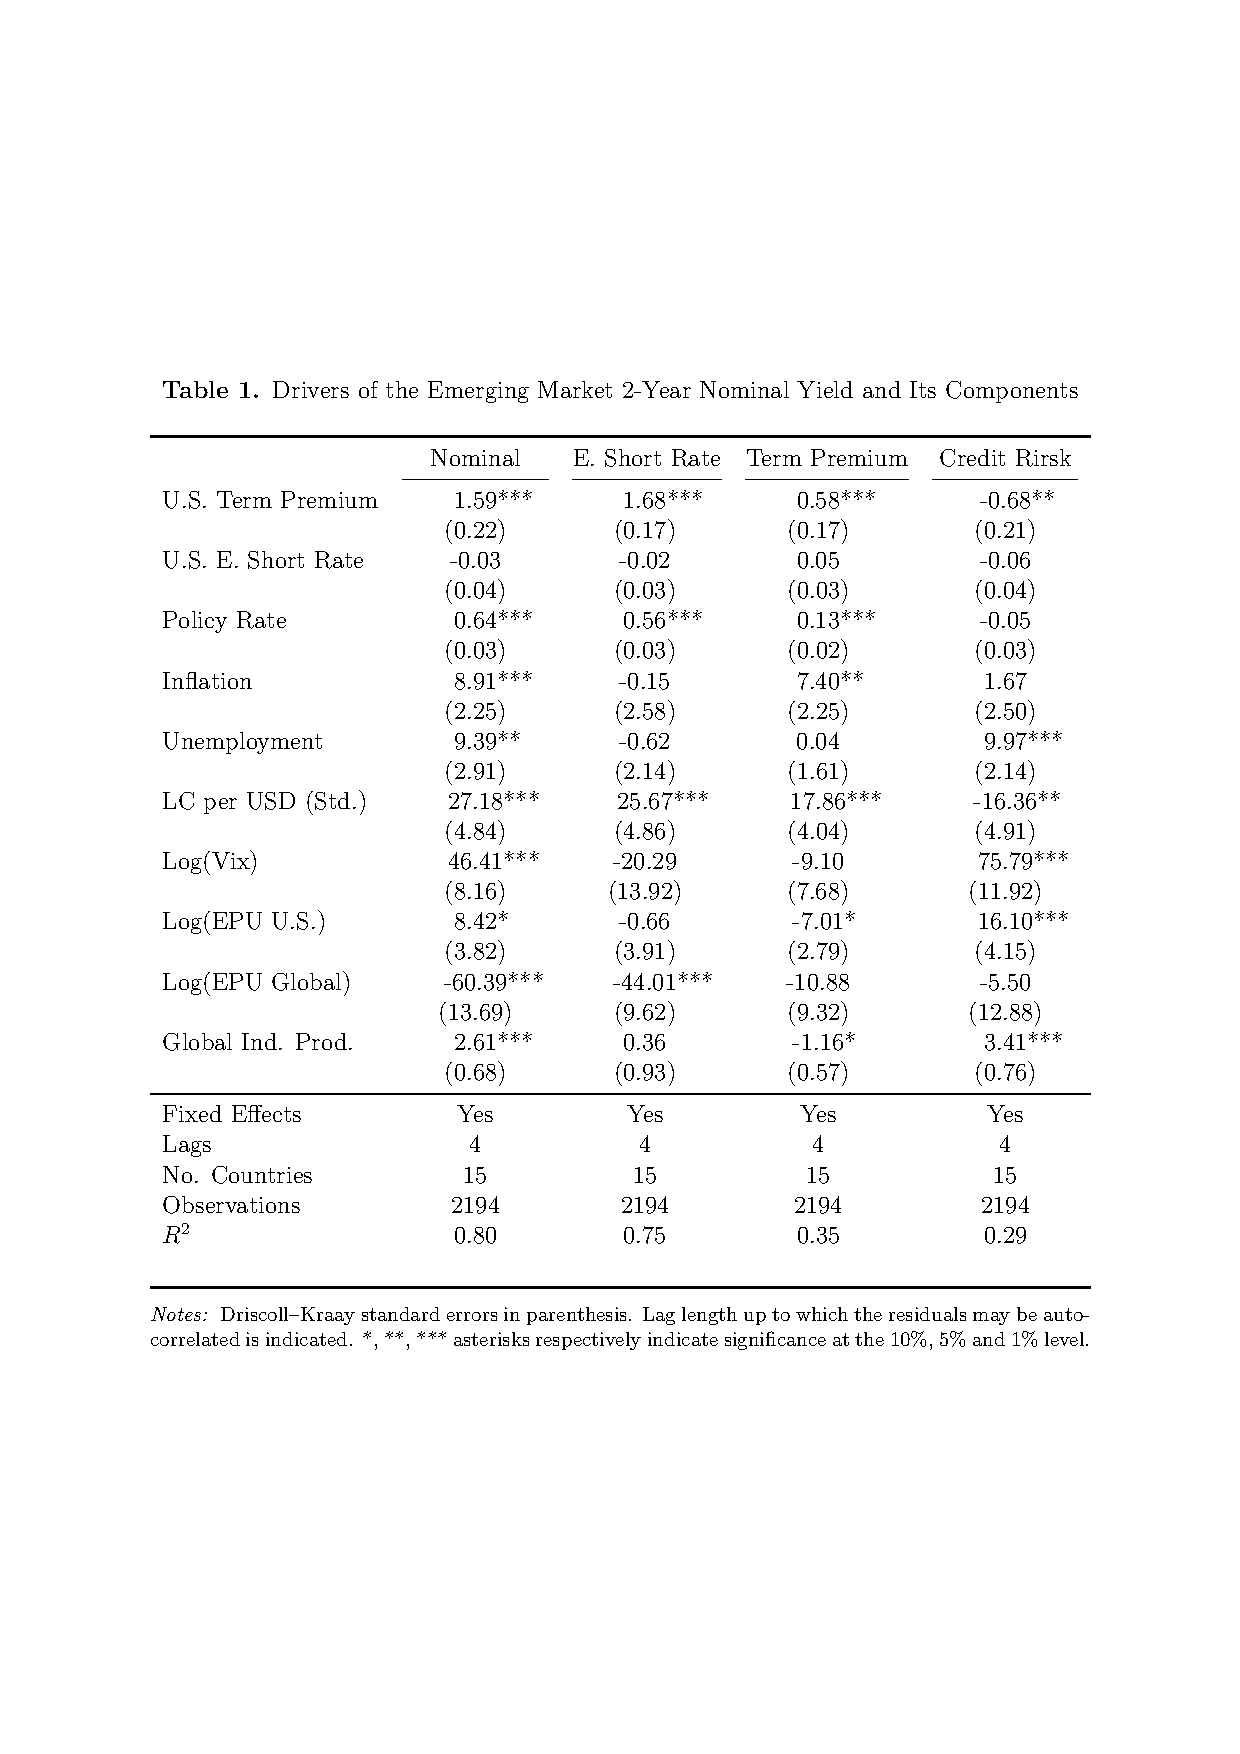
\includegraphics[trim={2cm 7.1cm 2cm 5cm},clip,height=1\textheight,width=0.85\textwidth]{../Tables/ycdcmp2y.pdf}};
%	%\draw[step=1cm,gray,very thin] (-4,-4) grid (6,6);
%	\draw[red,thick] (-6,1.6) rectangle (6,2.6);
%	\end{tikzpicture}
%\end{center}
%%\begin{figure}[!htbp]
%%	\begin{center} % trim removes: left, down, right, top
%%		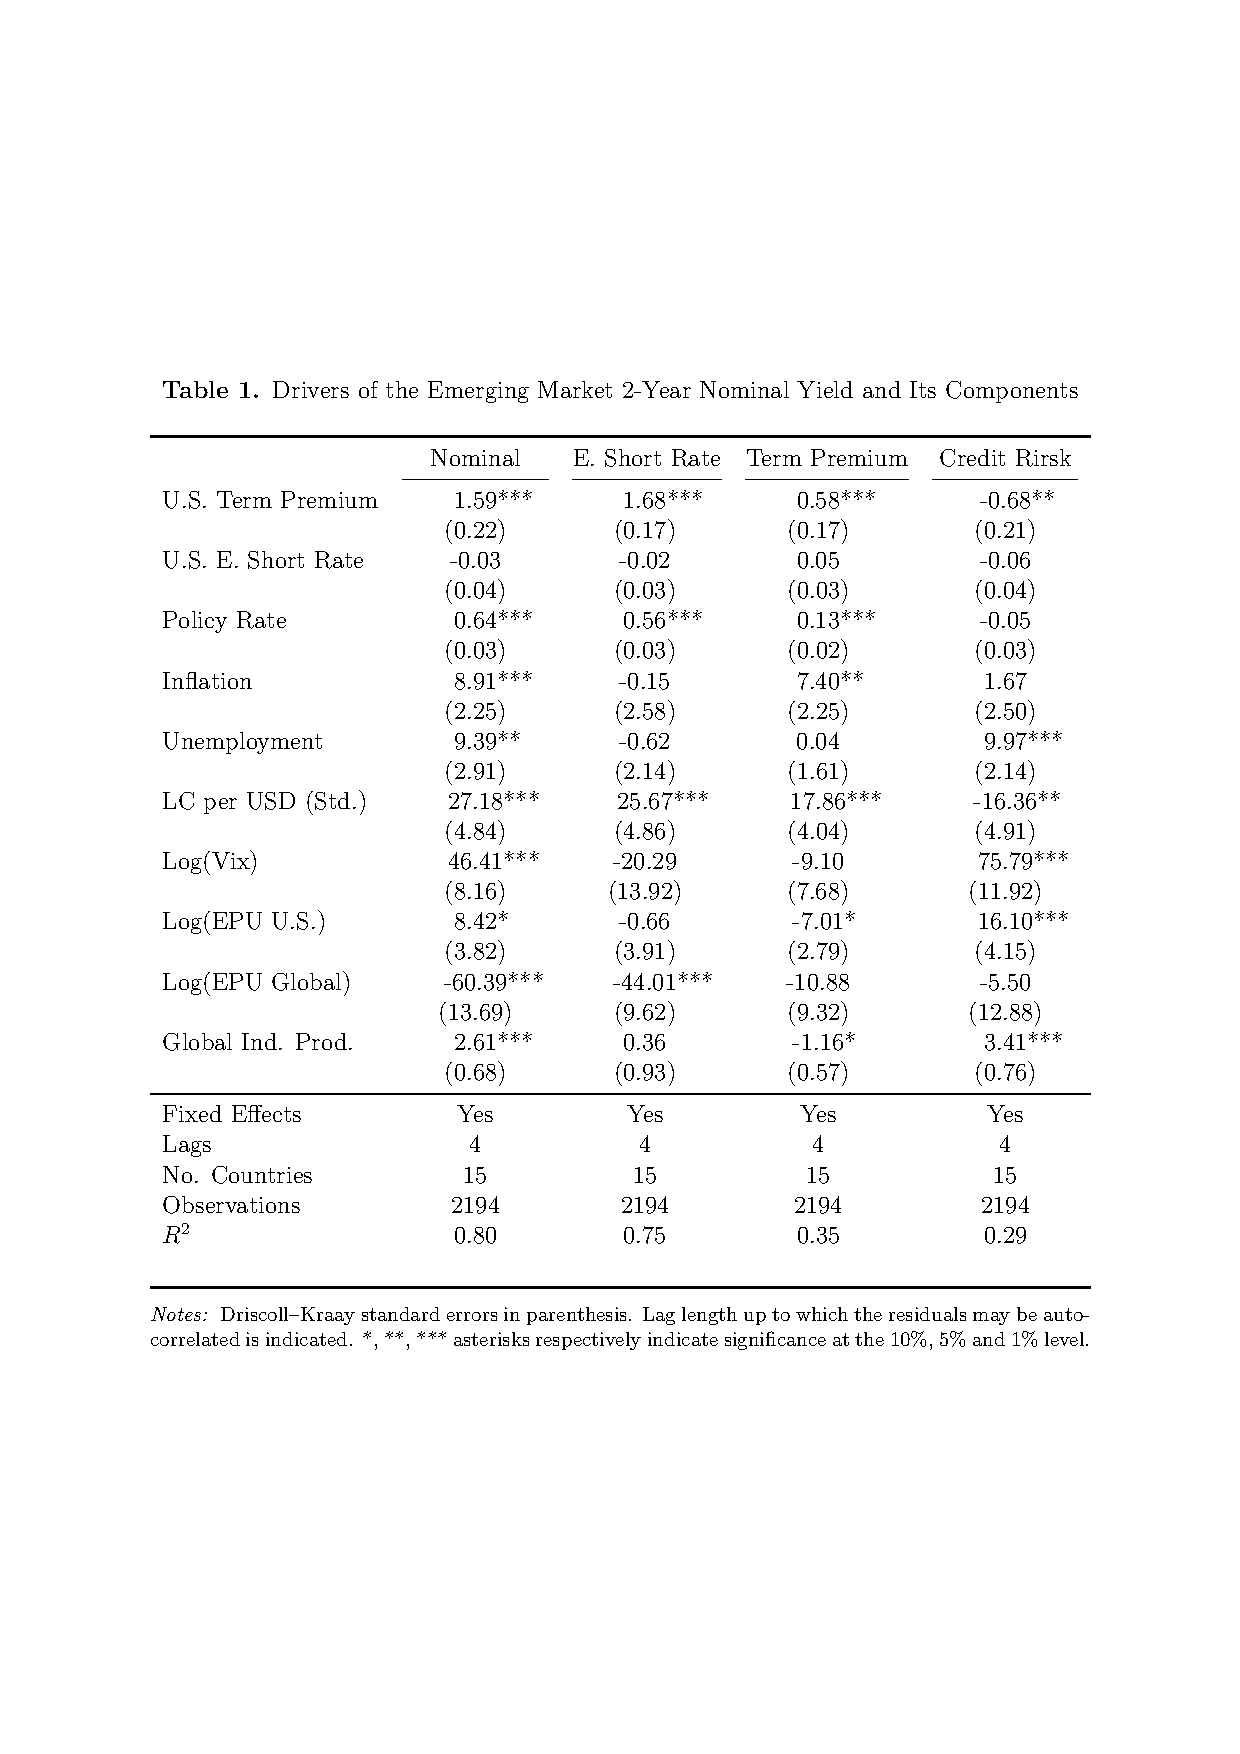
\includegraphics[trim={2cm 7.1cm 2cm 5cm},clip, width=0.85\textwidth,height=1\textheight]{../Tables/ycdcmp2y.pdf}
%%		\par\end{center}
%%\end{figure}
%\end{frame}
%
%\begin{frame}
%%	\frametitle{EM Term Premium and Inflation Uncertainty}
%\vspace{-0.8cm}
%\begin{center}
%	\begin{tikzpicture}
%	\node (table) at (0,0)
%	{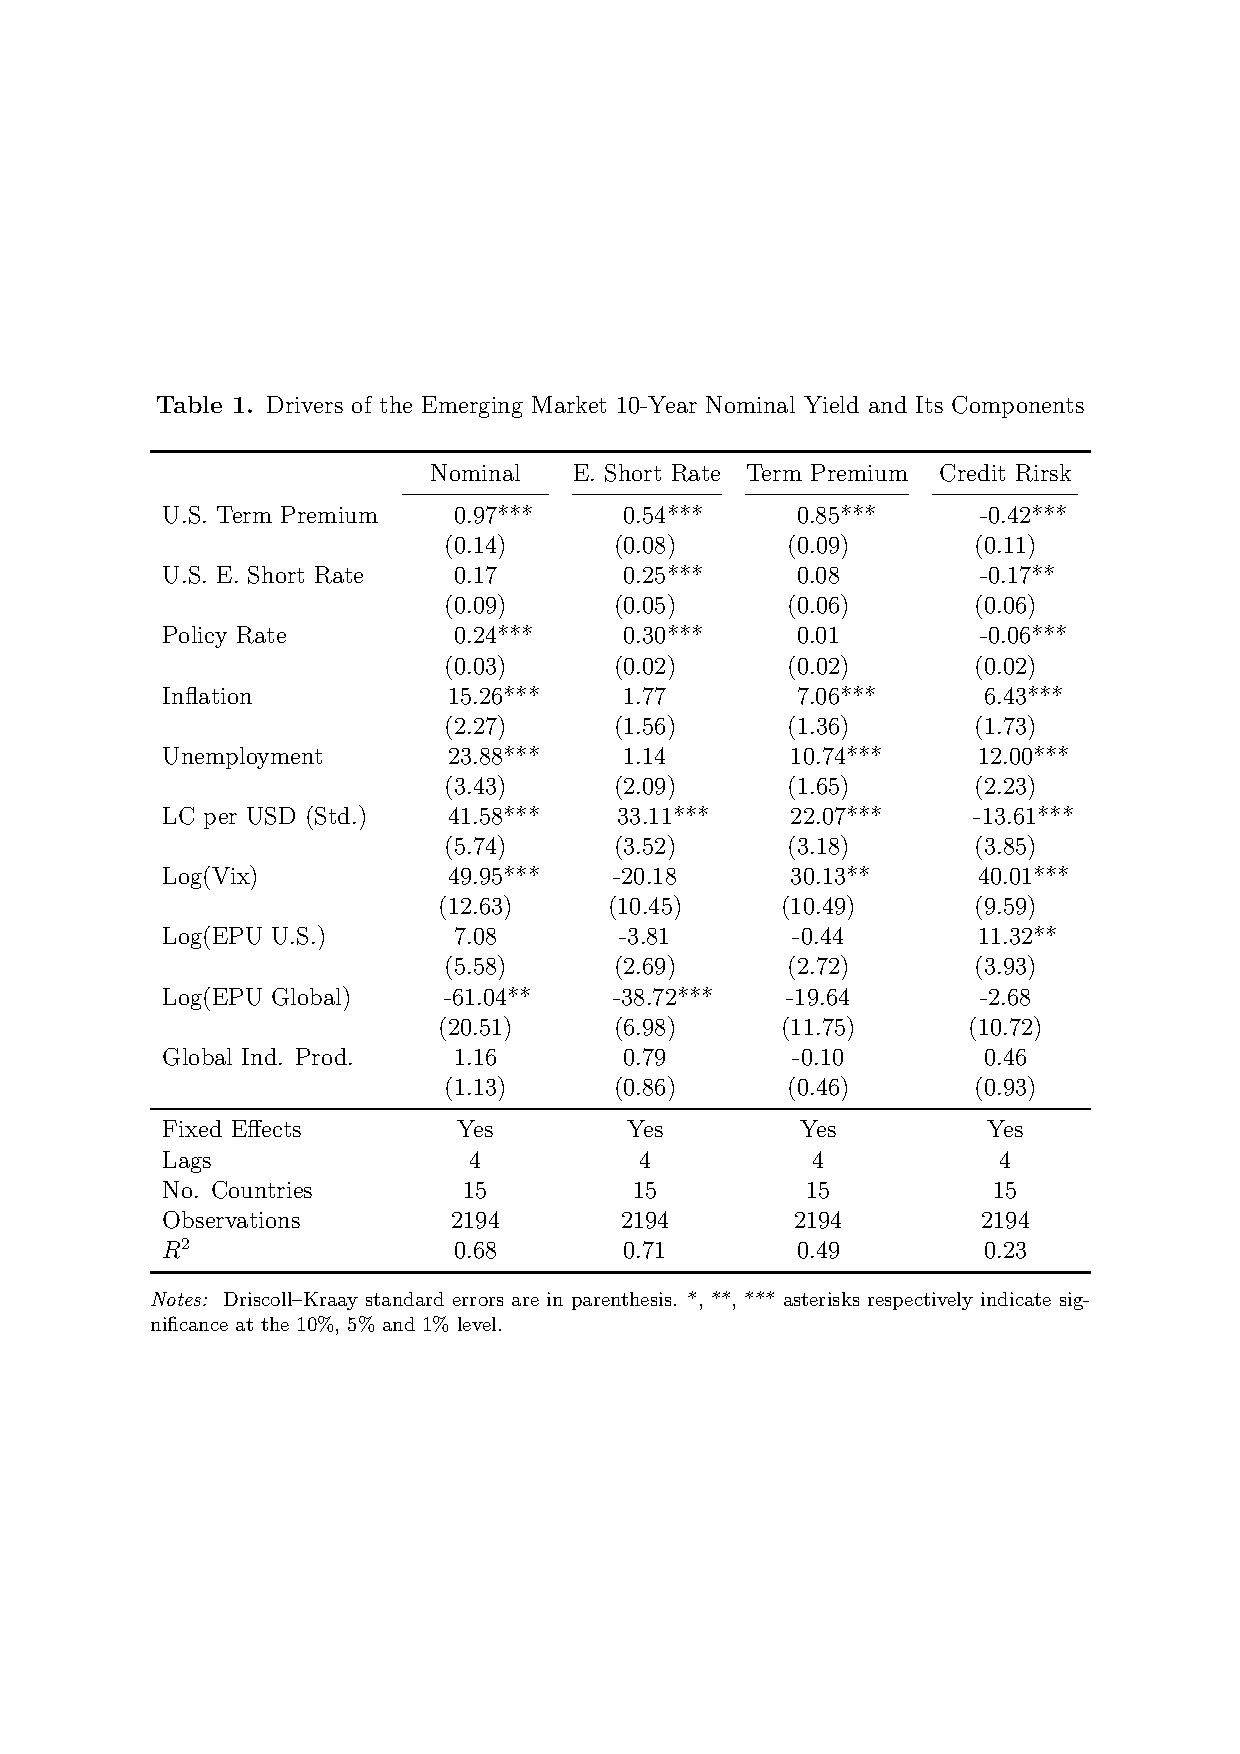
\includegraphics[trim={2cm 7.1cm 2cm 5cm},clip,height=1\textheight,width=0.85\textwidth]{../Tables/ycdcmp10y.pdf}};
%	%\draw[step=1cm,gray,very thin] (-4,-4) grid (6,6);
%	\draw[red,thick] (-6,1.6) rectangle (6,2.6);
%	\end{tikzpicture}
%\end{center}
%\end{frame}

{%
	\setbeamertemplate{frame footer}{See \cite{Kuttner:2001,GSS:2005a,Swanson:2018,NakamuraSteinsson:2018JEP}}
\begin{frame}
\frametitle{U.S. Monetary Policy Surprises}

Identification:
\begin{itemize}
	\item Asset price changes in 2-hour windows around FOMC meetings % since 2000
\end{itemize}

Surprises:
	\begin{itemize}
		\item \alert{Target}: federal funds futures contracts
		\item \alert{Forward guidance}: residual of Eurodollar ED8 yield on target surprise
		\item \alert{Asset purchases}: residual of 10Y Treasury yield on target and forward guidance surprises starting in 2009
	\end{itemize}

\end{frame}
}

\begin{frame}
\frametitle{U.S. Monetary Policy Effects on EM Yields}
%\vspace{-1cm}
Panel local projections:
\begin{equation*} \label{eq:uPanelLP}
	\eqpanelLP
\end{equation*}	% \ref{eq:nPanelLP}
%\vspace{-0.7cm}
\begin{itemize}
\item \(\yld_{\idxspnl}\): 10- and 2-year nominal EM yields and their components
\item \(\idxh = 0, 1, \ldots, 45\) is horizon in days
\item \(\alpha_{\idxh,\idxi}\): country fixed effects
\item \(\epsilon^{j}_{\idxt}\): three types of \alert{monetary policy surprises}
\item \(\fx_{\idxspnllag}\): one-day lag in the exchange rate
\end{itemize}
\end{frame}
\note{Evidence of delayed response in AE.}
\note{All responses are assessed relative to a one basis point reduction (an easing) in any of the surprises.}
\note{DK SE, 90\% confidence bands}

\begin{frame}[label=TargetEM]
\frametitle{Effects of Target Surprises}
\begin{figure}[!htbp]
\begin{center} % trim removes: left, down, right, top
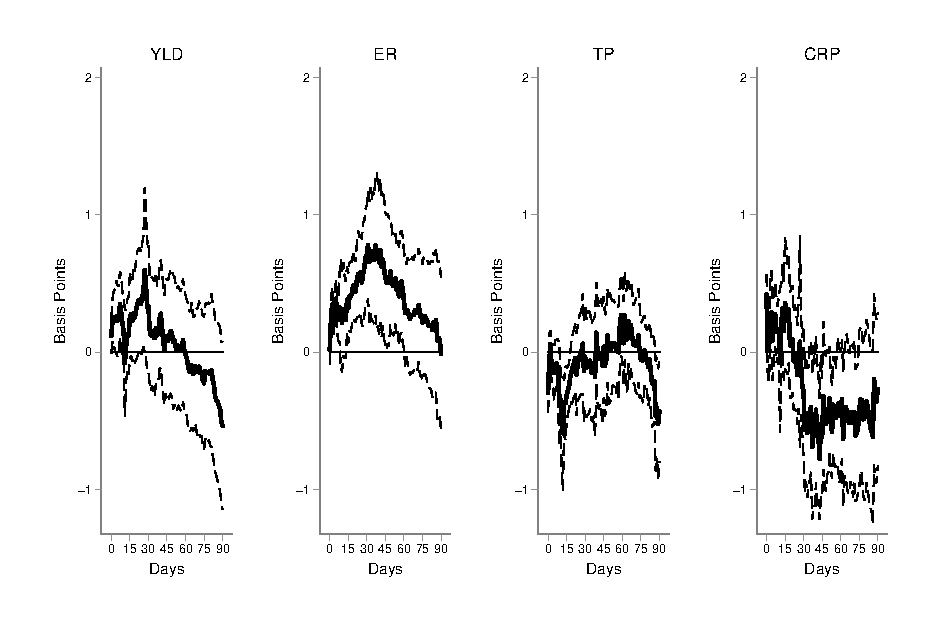
\includegraphics[trim={0cm 0cm 0cm 0cm},clip,height=0.45\textheight,width=0.85\linewidth]{../Figures/LPs/LagDep-FX/Target/EM/TargetEMnomyptpphi120m.eps}
\par\end{center}
\end{figure}
\vspace{-0.5cm}
\begin{figure}[!htbp]
\begin{center} % trim removes: left, down, right, top
\includegraphics[trim={0cm 0cm 0cm 0.76cm},clip,height=0.45\textheight,width=0.85\linewidth]{../Figures/LPs/LagDep-FX/Target/EM/TargetEMnomyptpphi24m.eps}
\par\end{center}
\end{figure}
\begin{textblock*}{8mm}(10mm,30mm)
\small 10Y
\end{textblock*}
\begin{textblock*}{8mm}(10mm,65mm)
\small 2Y
\end{textblock*}
\begin{textblock*}{5cm}(1.07\textwidth,0.65\textheight)
\hyperlink{TargetUS}{\beamergotobutton{US}}
\end{textblock*}
\end{frame}

\begin{frame}[label=FGEMpre]
\frametitle{Effects of Forward Guidance Surprises: Pre-GFC}
\begin{figure}[!htbp]
	\begin{center} % trim removes: left, down, right, top
		\includegraphics[trim={0cm 0cm 0cm 0cm},clip,height=0.45\textheight,width=0.85\linewidth]{../Figures/LPs/LagDep-FX/Path/EM/PathEMnomyptpphi120mPre.eps}
		\par\end{center}
\end{figure}
\vspace{-0.5cm}
\begin{figure}[!htbp]
	\begin{center} % trim removes: left, down, right, top
		\includegraphics[trim={0cm 0cm 0cm 0.76cm},clip,height=0.45\textheight,width=0.85\linewidth]{../Figures/LPs/LagDep-FX/Path/EM/PathEMnomyptpphi24mPre.eps}
		\par\end{center}
\end{figure}
\begin{textblock*}{8mm}(10mm,30mm)
	\small 10Y
\end{textblock*}
\begin{textblock*}{8mm}(10mm,65mm)
	\small 2Y
\end{textblock*}
\begin{textblock*}{5cm}(1.07\textwidth,0.65\textheight)
	\hyperlink{FGUSpre}{\beamergotobutton{US}}
\end{textblock*}
\end{frame}

\begin{frame}[label=FGEMpost]
\frametitle{Effects of Forward Guidance Surprises: Post-GFC}
\begin{figure}[!htbp]
\begin{center} % trim removes: left, down, right, top
\includegraphics[trim={0cm 0cm 0cm 0cm},clip,height=0.45\textheight,width=0.85\linewidth]{../Figures/LPs/LagDep-FX/Path/EM/PathEMnomyptpphi120mPost.eps}
\par\end{center}
\end{figure}
\vspace{-0.5cm}
\begin{figure}[!htbp]
\begin{center} % trim removes: left, down, right, top
\includegraphics[trim={0cm 0cm 0cm 0.76cm},clip,height=0.45\textheight,width=0.85\linewidth]{../Figures/LPs/LagDep-FX/Path/EM/PathEMnomyptpphi24mPost.eps}
\par\end{center}
\end{figure}
\begin{textblock*}{8mm}(10mm,30mm)
\small 10Y
\end{textblock*}
\begin{textblock*}{8mm}(10mm,65mm)
\small 2Y
\end{textblock*}
\begin{textblock*}{5cm}(1.07\textwidth,0.65\textheight)
\hyperlink{FGUSpost}{\beamergotobutton{US}}
\end{textblock*}
\end{frame}

\begin{frame}[label=LSAPEM]
\frametitle{Effects of Asset Purchase Surprises}
\begin{figure}[!htbp]
\begin{center} % trim removes: left, down, right, top
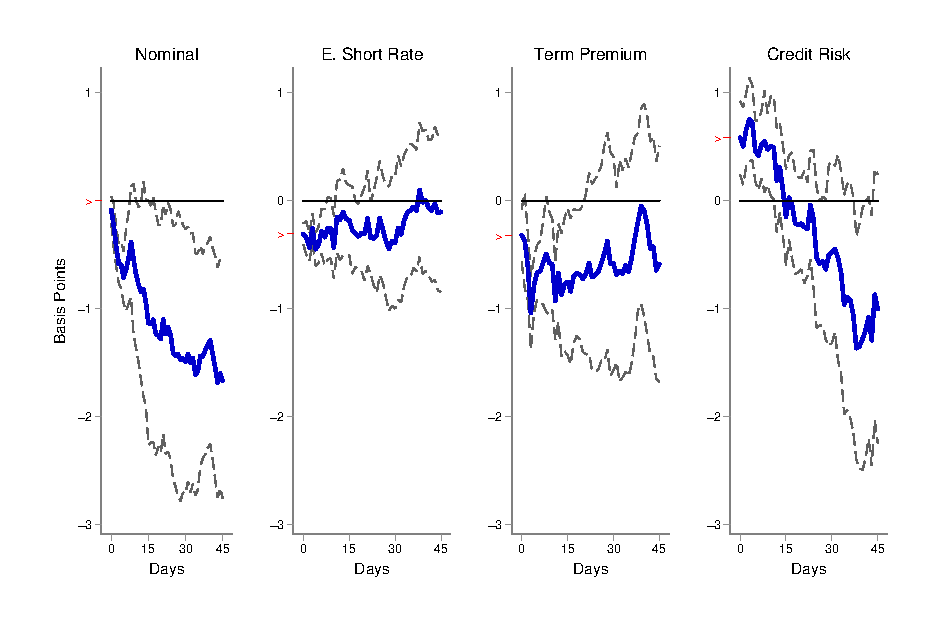
\includegraphics[trim={0cm 0cm 0cm 0cm},clip,height=0.45\textheight,width=0.85\linewidth]{../Figures/LPs/LagDep-FX/LSAP/EM/LSAPEMnomyptpphi120m.eps}
\par\end{center}
\end{figure}
\vspace{-0.5cm}
\begin{figure}[!htbp]
\begin{center} % trim removes: left, down, right, top
\includegraphics[trim={0cm 0cm 0cm 0.76cm},clip,height=0.45\textheight,width=0.85\linewidth]{../Figures/LPs/LagDep-FX/LSAP/EM/LSAPEMnomyptpphi24m.eps}
\par\end{center}
\end{figure}
\begin{textblock*}{8mm}(10mm,30mm)
\small 10Y
\end{textblock*}
\begin{textblock*}{8mm}(10mm,65mm)
\small 2Y
\end{textblock*}
\begin{textblock*}{5cm}(1.07\textwidth,0.65\textheight)
\hyperlink{LSAPUS}{\beamergotobutton{US}}
\end{textblock*}
\end{frame}

\section{Conclusions}

\begin{frame}
\frametitle{Conclusions}

\alert{Three}-part decomposition of EM yields
\begin{itemize}
\item Average expected short rate \item Term premium \item Credit risk compensation
\end{itemize}

U.S. monetary policy \alert{spillovers}
\begin{enumerate}
\item Responses are economically significant yet delayed
\item Reassessment of policy rate expectations, repricing of risks
\item Evidence of a yield curve channel since 2008
\end{enumerate}

\end{frame}
\note{YC channel: EM monetary autonomy decreases along the yield curve and involves the credit risk compensation.}
\note{To understand comovement, I propose a decomposition of EM yields.}
\note{Extensions: nominal-real decompositions, jumps.}

\begin{frame}[standout]
Appendix
\end{frame}

\appendix

\begin{frame}[label=tpCI]
%	\frametitle{Components: Term Premium}
\begin{center}							% center the figure inside the minipage
\includegraphics[trim={0cm 0cm 0cm 0cm},clip,height=0.95\textheight,width=\linewidth]{../Figures/Estimation/bsl_tp_CI_10y_V1.eps} \\
\end{center}
\begin{textblock*}{5cm}(0.97\textwidth,1.05\textheight)
\hyperlink{YldDcmp}{\beamerreturnbutton{Decomposition}}
\end{textblock*}
\end{frame}
\note{Survey-Based Term Premium Estimates}
\note{EM TP are time-varying.}
\note{Sensible TP estimates, mostly positive; fluctuate between 0\% and 5\%.}
\note{Sometimes they comove.}

\begin{frame}[label=crcCI]
%\frametitle{Components: Credit Risk Compensation}
\begin{center}							% center the figure inside the minipage
\includegraphics[trim={0cm 0cm 0cm 0cm},clip,height=0.95\textheight,width=\linewidth]{../Figures/Estimation/bsl_cr_CI_10y_V1.eps} \\
\end{center}
\begin{textblock*}{5cm}(0.97\textwidth,1.05\textheight)
\hyperlink{YldDcmp}{\beamerreturnbutton{Decomposition}}
\end{textblock*}
\end{frame}

\begin{frame}[label=DYindex]
\frametitle{EM Yields Comovement}
\begin{figure}[!htbp]
	\begin{center} % trim removes: left, down, right, top
		\includegraphics[trim={0cm 0cm 0cm 0cm},clip,height=0.8\textheight,width=0.85\linewidth]{../Figures/Estimation/dy_index_dn_data.eps}
		\par\end{center}
\end{figure}
\begin{textblock*}{10cm}(45mm,83mm)
	\footnotesize Connectedness Index \citep{DieboldYilmaz:2014}
\end{textblock*}
\begin{textblock*}{5cm}(1.02\textwidth,0.55\textheight)
	\hyperlink{RollingCorr}{\beamergotobutton{Rolling Corr.}}
\end{textblock*}
\end{frame}

%\begin{frame}[label=RollingCorr]
%\frametitle{EM Yields Comovement}
%\begin{figure}[!htbp]
%\begin{center} % trim removes: left, down, right, top
%	\includegraphics[trim={0cm 0cm 0cm 0cm},clip,height=0.8\textheight,width=0.85\linewidth]{../Figures/Estimation/rolling_dn_data.eps}
%	\par\end{center}
%\end{figure}
%\begin{textblock*}{10cm}(67.5mm,83mm)
%\footnotesize Rolling Correlations
%\end{textblock*}
%\begin{textblock*}{5cm}(1.02\textwidth,0.55\textheight)
%\hyperlink{DYindex}{\beamergotobutton{D-Y Index}}
%\end{textblock*}
%\end{frame}

\begin{frame}[label=TargetUS]
\frametitle{Effects of Target Surprises}
\begin{figure}[!htbp]
\begin{center} % trim removes: left, down, right, top
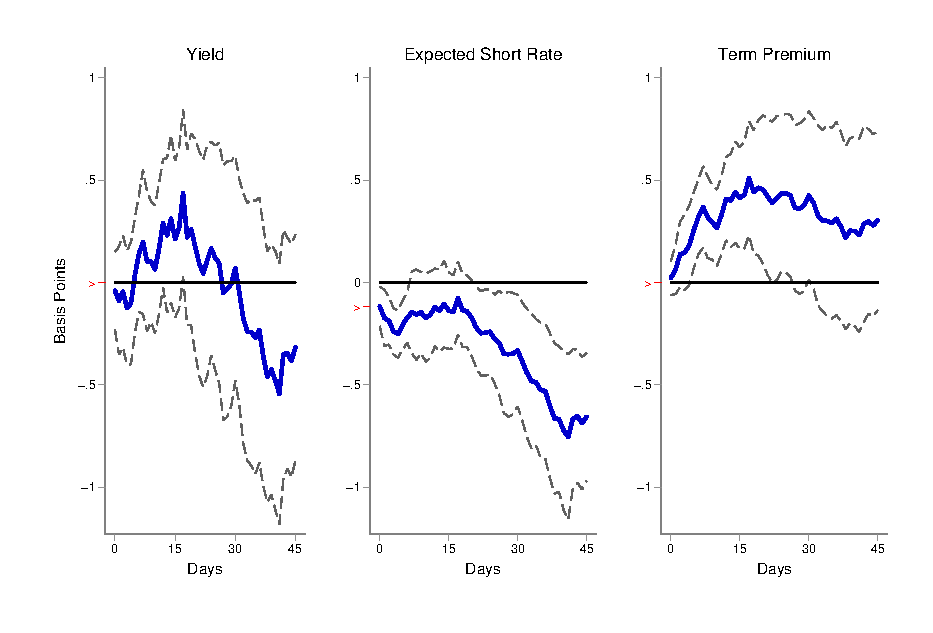
\includegraphics[trim={0cm 0cm 0cm 0cm},clip,height=0.45\textheight,width=0.85\linewidth]{../Figures/LPs/LagDep-FX/Target/US/DCMP/TargetUSDnomyptp120m.eps}
\par\end{center}
\end{figure}
\vspace{-0.5cm}
\begin{figure}[!htbp]
\begin{center} % trim removes: left, down, right, top
\includegraphics[trim={0cm 0cm 0cm 0.76cm},clip,height=0.45\textheight,width=0.85\linewidth]{../Figures/LPs/LagDep-FX/Target/US/DCMP/TargetUSDnomyptp24m.eps}
\par\end{center}
\end{figure}
\begin{textblock*}{8mm}(10mm,30mm)
\small 10Y
\end{textblock*}
\begin{textblock*}{8mm}(10mm,65mm)
\small 2Y
\end{textblock*}
\begin{textblock*}{5cm}(1.07\textwidth,0.65\textheight)
\hyperlink{TargetEM}{\beamerreturnbutton{EM}}
\end{textblock*}
\end{frame}

\begin{frame}[label=FGUSpre]
\frametitle{Effects of Forward Guidance Surprises: Pre-GFC}
\begin{figure}[!htbp]
	\begin{center} % trim removes: left, down, right, top
		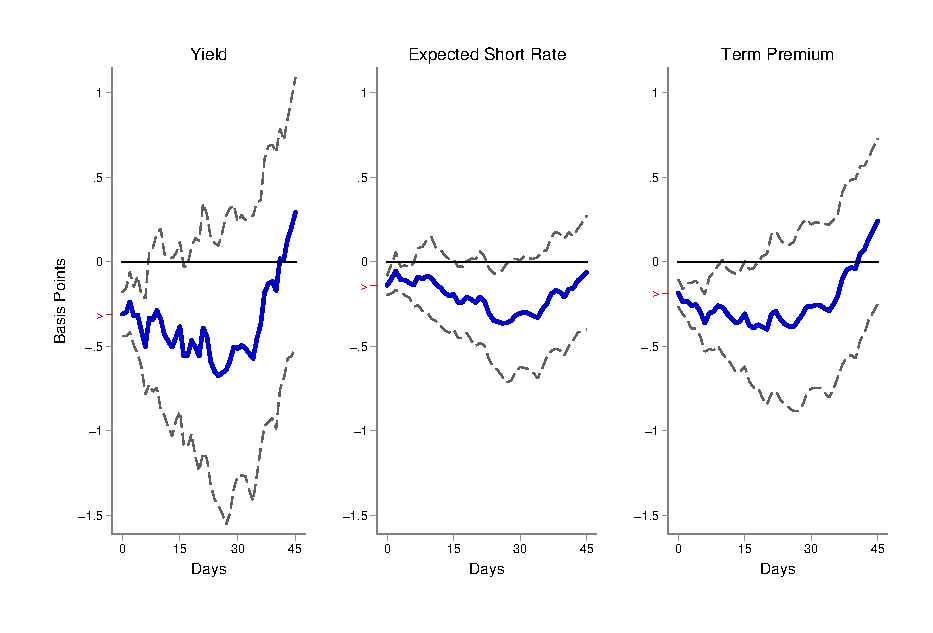
\includegraphics[trim={0cm 0cm 0cm 0cm},clip,height=0.45\textheight,width=0.85\linewidth]{../Figures/LPs/LagDep-FX/Path/US/DCMP/PathUSDnomyptp120mPre.eps}
		\par\end{center}
\end{figure}
\vspace{-0.5cm}
\begin{figure}[!htbp]
	\begin{center} % trim removes: left, down, right, top
		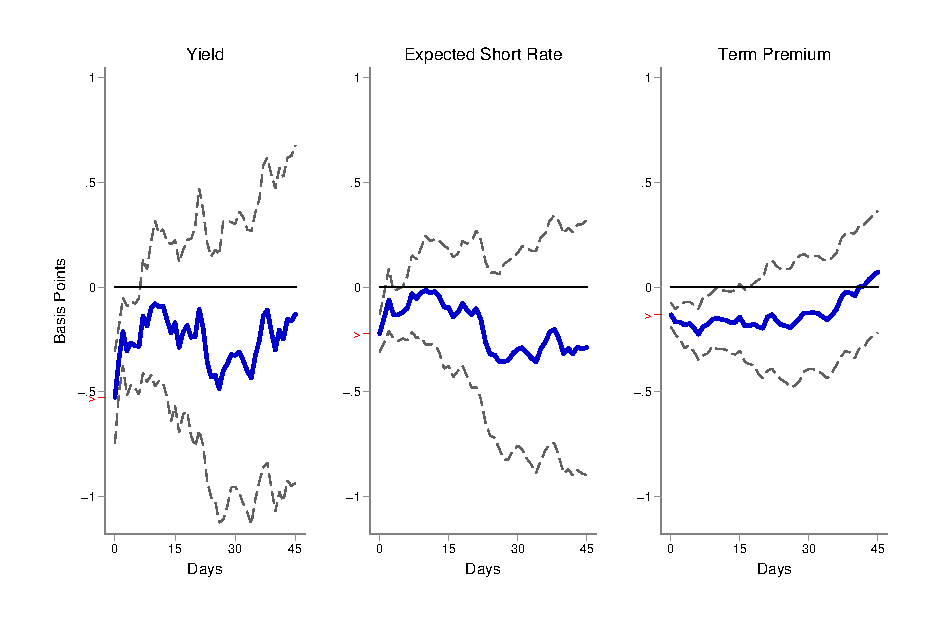
\includegraphics[trim={0cm 0cm 0cm 0.76cm},clip,height=0.45\textheight,width=0.85\linewidth]{../Figures/LPs/LagDep-FX/Path/US/DCMP/PathUSDnomyptp24mPre.eps}
		\par\end{center}
\end{figure}
\begin{textblock*}{8mm}(10mm,30mm)
	\small 10Y
\end{textblock*}
\begin{textblock*}{8mm}(10mm,65mm)
	\small 2Y
\end{textblock*}
\begin{textblock*}{5cm}(1.07\textwidth,0.65\textheight)
	\hyperlink{FGEMpre}{\beamerreturnbutton{EM}}
\end{textblock*}
\end{frame}

\begin{frame}[label=FGUSpost]
\frametitle{Effects of Forward Guidance Surprises: Post-GFC}
\begin{figure}[!htbp]
\begin{center} % trim removes: left, down, right, top
\includegraphics[trim={0cm 0cm 0cm 0cm},clip,height=0.45\textheight,width=0.85\linewidth]{../Figures/LPs/LagDep-FX/Path/US/DCMP/PathUSDnomyptp120mPost.eps}
\par\end{center}
\end{figure}
\vspace{-0.5cm}
\begin{figure}[!htbp]
\begin{center} % trim removes: left, down, right, top
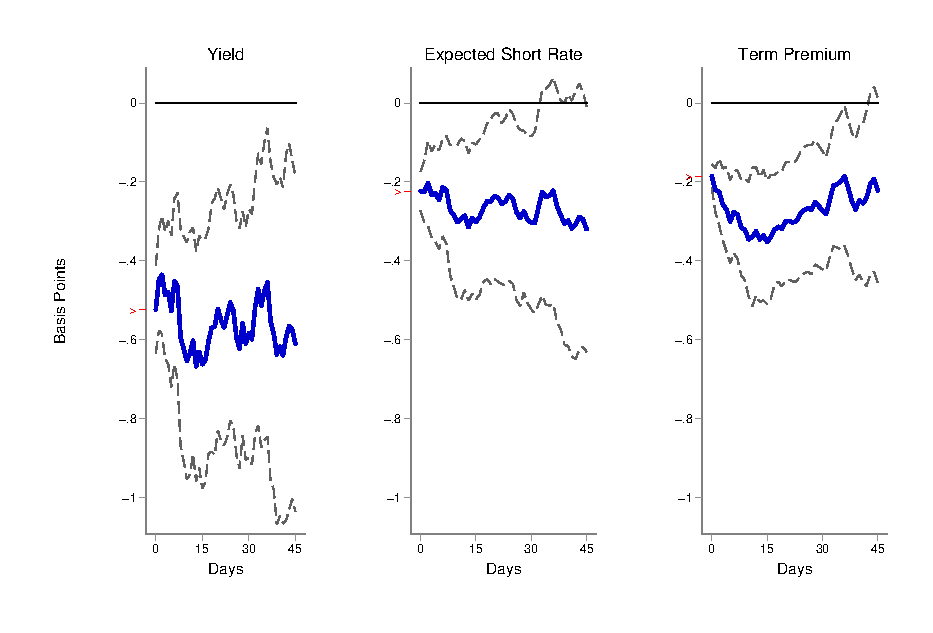
\includegraphics[trim={0cm 0cm 0cm 0.76cm},clip,height=0.45\textheight,width=0.85\linewidth]{../Figures/LPs/LagDep-FX/Path/US/DCMP/PathUSDnomyptp24mPost.eps}
\par\end{center}
\end{figure}
\begin{textblock*}{8mm}(10mm,30mm)
\small 10Y
\end{textblock*}
\begin{textblock*}{8mm}(10mm,65mm)
\small 2Y
\end{textblock*}
\begin{textblock*}{5cm}(1.07\textwidth,0.65\textheight)
\hyperlink{FGEMpost}{\beamerreturnbutton{EM}}
\end{textblock*}
\end{frame}

\begin{frame}[label=LSAPUS]
\frametitle{Effects of Asset Purchase Surprises}
\begin{figure}[!htbp]
\begin{center} % trim removes: left, down, right, top
\includegraphics[trim={0cm 0cm 0cm 0cm},clip,height=0.45\textheight,width=0.85\linewidth]{../Figures/LPs/LagDep-FX/LSAP/US/DCMP/LSAPUSDnomyptp120m.eps}
\par\end{center}
\end{figure}
\vspace{-0.5cm}
\begin{figure}[!htbp]
\begin{center} % trim removes: left, down, right, top
\includegraphics[trim={0cm 0cm 0cm 0.76cm},clip,height=0.45\textheight,width=0.85\linewidth]{../Figures/LPs/LagDep-FX/LSAP/US/DCMP/LSAPUSDnomyptp24m.eps}
\par\end{center}
\end{figure}
\begin{textblock*}{8mm}(10mm,30mm)
\small 10Y
\end{textblock*}
\begin{textblock*}{8mm}(10mm,65mm)
\small 2Y
\end{textblock*}
\begin{textblock*}{5cm}(1.07\textwidth,0.65\textheight)
\hyperlink{LSAPEM}{\beamerreturnbutton{EM}}
\end{textblock*}
\end{frame}

%---------------------------------------------------------------
% Sources
%---------------------------------------------------------------
% Tips in general
% https://en.wikibooks.org/wiki/LaTeX/Presentations
%https://tex.stackexchange.com/questions/12328/how-can-i-use-todonotes-with-beamer
% Insert links to slides
% https://latex.org/forum/viewtopic.php?t=4594
% Place button of link on slide
%https://tex.stackexchange.com/questions/50643/hyperlink-button-in-an-exact-position
% Make figures visible
%https://stackoverflow.com/questions/4683093/beamer-how-to-show-images-as-step-by-step-images
% Multicolumn and multirow
%https://tex.stackexchange.com/questions/156219/proper-centering-with-cmidrule-and-multi-row-and-column

% Metropolis
%http://mirrors.ibiblio.org/CTAN/macros/latex/contrib/beamer-contrib/themes/metropolis/doc/metropolistheme.pdf
%https://github.com/matze/mtheme

% Code for hyperlinks
%[label=corr_10yr]
%\begin{textblock*}{3cm}(.9\textwidth,-.5\textheight)
%	\hyperlink{corr_10yr}{\beamergotobutton{10-Year TP}}
%\end{textblock*}
%
%\begin{textblock*}{3cm}(.9\textwidth,-.5\textheight)
%	\hyperlink{corr_10yr}{\beamerreturnbutton{10-Year TP}}
%\end{textblock*}

% Two-column frame template
%http://felix11h.github.io/blog/beamer-two-col



%\begin{frame}[allowframebreaks]{References}
\begin{frame}<presentation:0>
\bibliographystyle{abbrvnat} 
\bibliography{../../../References/library}
\end{frame}

\end{document}